\documentclass[journal]{IEEEtran}
\usepackage{times}

% numbers option provides compact numerical references in the text. 

\usepackage{graphics} % for pdf, bitmapped graphics files
\usepackage{epsfig} % for postscript graphics files
\usepackage{mathptmx} % assumes new font selection scheme installed
\usepackage{times} % assumes new font selection scheme installed
\usepackage{amsmath} % assumes amsmath package installed
\usepackage{amssymb}  % assumes amsmath package installed
%\usepackage{amsthm}
\usepackage{mathtools}
\usepackage{bm}
\usepackage{mathrsfs}
\usepackage{xcolor}
\usepackage{cite}
\usepackage{threeparttable}
\usepackage{multirow}
\usepackage{bigdelim}
\usepackage{algorithm}
\usepackage{algorithmicx}
\usepackage{algpseudocode}
\usepackage{graphicx}
\usepackage{subfigure}
\usepackage{comment}

\usepackage{amsmath}

\usepackage[numbers]{natbib}
\usepackage{multicol}
\usepackage[bookmarks=true]{hyperref}

\pdfinfo{
   /Author (Homer Simpson)
   /Title  (Robots: Our new overlords)
   /CreationDate (D:20101201120000)
   /Subject (Robots)
   /Keywords (Robots;Overlords)
}

\begin{document}


%\title{Theoretically Complete Solution to the Optimal Non-repetitive Coverage Task of Arbitrary Shape Object with Minimal Discontinuities for a Non-redundant Robot Manipulator}
\title{Non-revisiting Coverage Task with Minimal Discontinuities for Non-redundant Manipulators}



\author{Tong Yang, Jaime Valls Miro, Yue Wang$^*$ and Rong Xiong
\thanks{$^1$ Tong Yang, Yue Wang and Rong Xiong are with the State Key 
Laboratory of Industrial Control and Technology, Zhejiang University, P.R. China. 
}
\thanks{$^2$ Jaime Valls Miro is with the Centre for Autonomous Systems (CAS), University of Technology Sydney (UTS), Sydney, Australia.}
%\thanks{This work was supported by National Key R\&D Program of China (2018YFB1309300) National Nature Science Foundation of China (61903332, U1609210).}
\thanks{$^*$ Corresponding Author. \newline \indent
E-mail address: {\tt\small wangyue@iipc.zju.edu.cn}}
}

\maketitle

\begin{abstract}
A theoretically complete solution to the optimal Non-revisiting Coverage Path Planning (NCPP) problem of any arbitrarily-shaped 
object with a non-redundant manipulator is proposed in this work. 
Given topological graphs of surface cells corresponding to feasible and continuous manipulator configurations, 
the scheme is aimed at ensuring optimality with respect to the number of surface discontinuities,  
% without revisiting
%proved finitly solvable, and a mechanism to derive all topological solutions is proposed. However, the topological graph is created just based on some classical constraints of the manipulator, which is solvable only if all cells are simply-connected. 
and extends the existing provable solution attained for simply-connected configuration cell topologies to any arbitrary shape. 
This is typically classified through their genus, or the number of ``holes" 
%of all cells can be classified through their genus, while our previous work only proves the solvability of the simply-connected cells. 
which appear increasingly as configurations are further constrained with the introduction of additional metrics for the
 task at hand, e.g. manipulability thresholds, clearance from obstacles, end-effector orientations, tooling force/torque magnitudes, etc.
%and additional thresholds based on them determine the shape of the cells. 

%As such, the proposed work solves topological graphs created from any quality measurement, we consider the solvability of the cells with all possible genus. 

The novel contribution of this paper is to show that no matter what the resulting topological shapes from such quality cell constraints may be, the graph is finitely solvable, and a multi-stage iterative solver is designed to find all such optimal solutions. 
\end{abstract}

\IEEEpeerreviewmaketitle
\section{Introduction}
Full coverage of the surface of a given object with non-redundant manipulators is embodied in tasks such as 
automatic polishing, deburring, painting or surface inspection, where the need for non-repetitive path planning 
is paramount to avoid over revisiting. 

The kinematic relationship of a typical manipulator makes mapping between work- and joint-space 
non-bijective~\cite{lavalle2006planning}, which in effect drives coverage paths to be traditionally carried out in the former to 
ensure no revisiting of points in the surface~\cite{Oriolo2005Motion}. However, in further pursuing motions 
where the manipulator may minimise the number of reconfigurations is obliged to undertake to follow a desirable 
continous end-effector (EE) path, a global optimal cellular decomposition problem in joint-space has been 
proposed to incur joint-space partitions with minimum sets~\cite{Yang2020Cellular}. This is illustrated in 
the example shown by Fig.~\ref{fig:TMech}: the external surface of a wok-like object is inspected by a 
non-redundant manipulator. Points on the surface can be reached by a variety of robot configurations. 
The three solid colour cells shown in Fig.~\ref{fig:TMech_config_cells} illustrate poses of disjoint sets reachable 
as a continous set by a given configuration, visually seen by the different colours. These cells become the elements 
on a topological graph Fig.~\ref{fig:TMech_topo_graph}, where each possible colour of a cell is recorded. 
A cellular decomposition splits and merges the cells to transform the process into that of painting all points in the 
graph with one of the possible colours, driven by attaining a minimum set which equates to least number of EE lift-offs. 
One such optimal solution with 2 lift-offs is illustrated in Fig.~\ref{fig:TMech_solution}, whereby any arbitrary 
continuous path within a colour surface area will result in maxium joint continuity of the global path. 
The addition of obstacles and the relative pose of robot and object further condition the final solution. 
For further details please refer to~\cite{Yang2020Cellular}. 

\begin{comment}
\begin{figure}[t]
\centering
\subfigure[Left: Four different kinds of configurations. Middle: Their reachable areas on the mesh.
 Right: The topological graph which contains non simply-connected cells. ]{
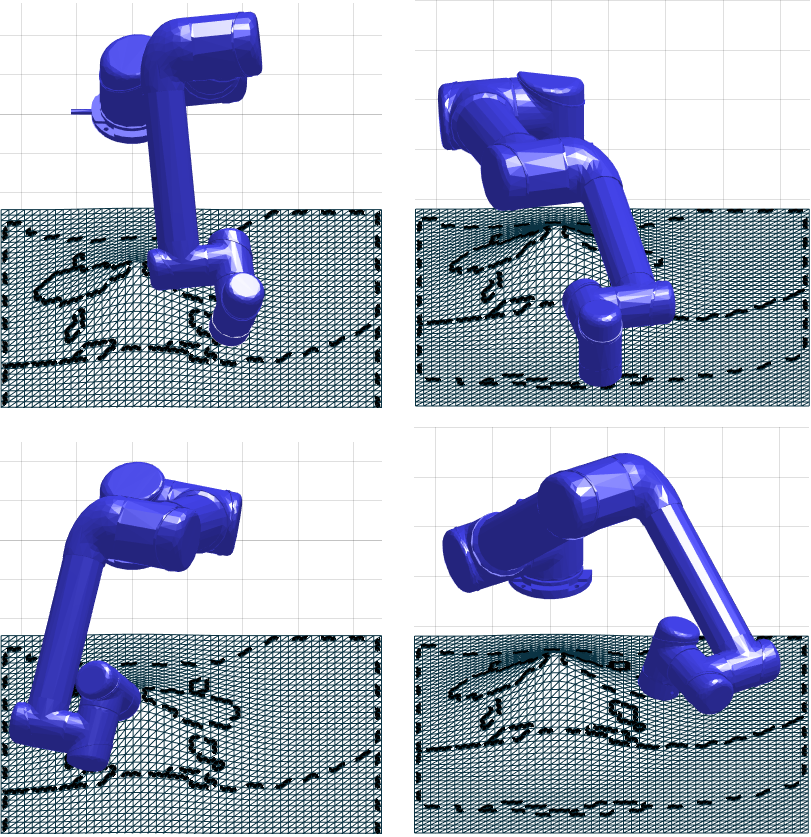
\includegraphics[width = 0.15\textwidth]{figures/hill_exp/0_06/hill_demo_comb}
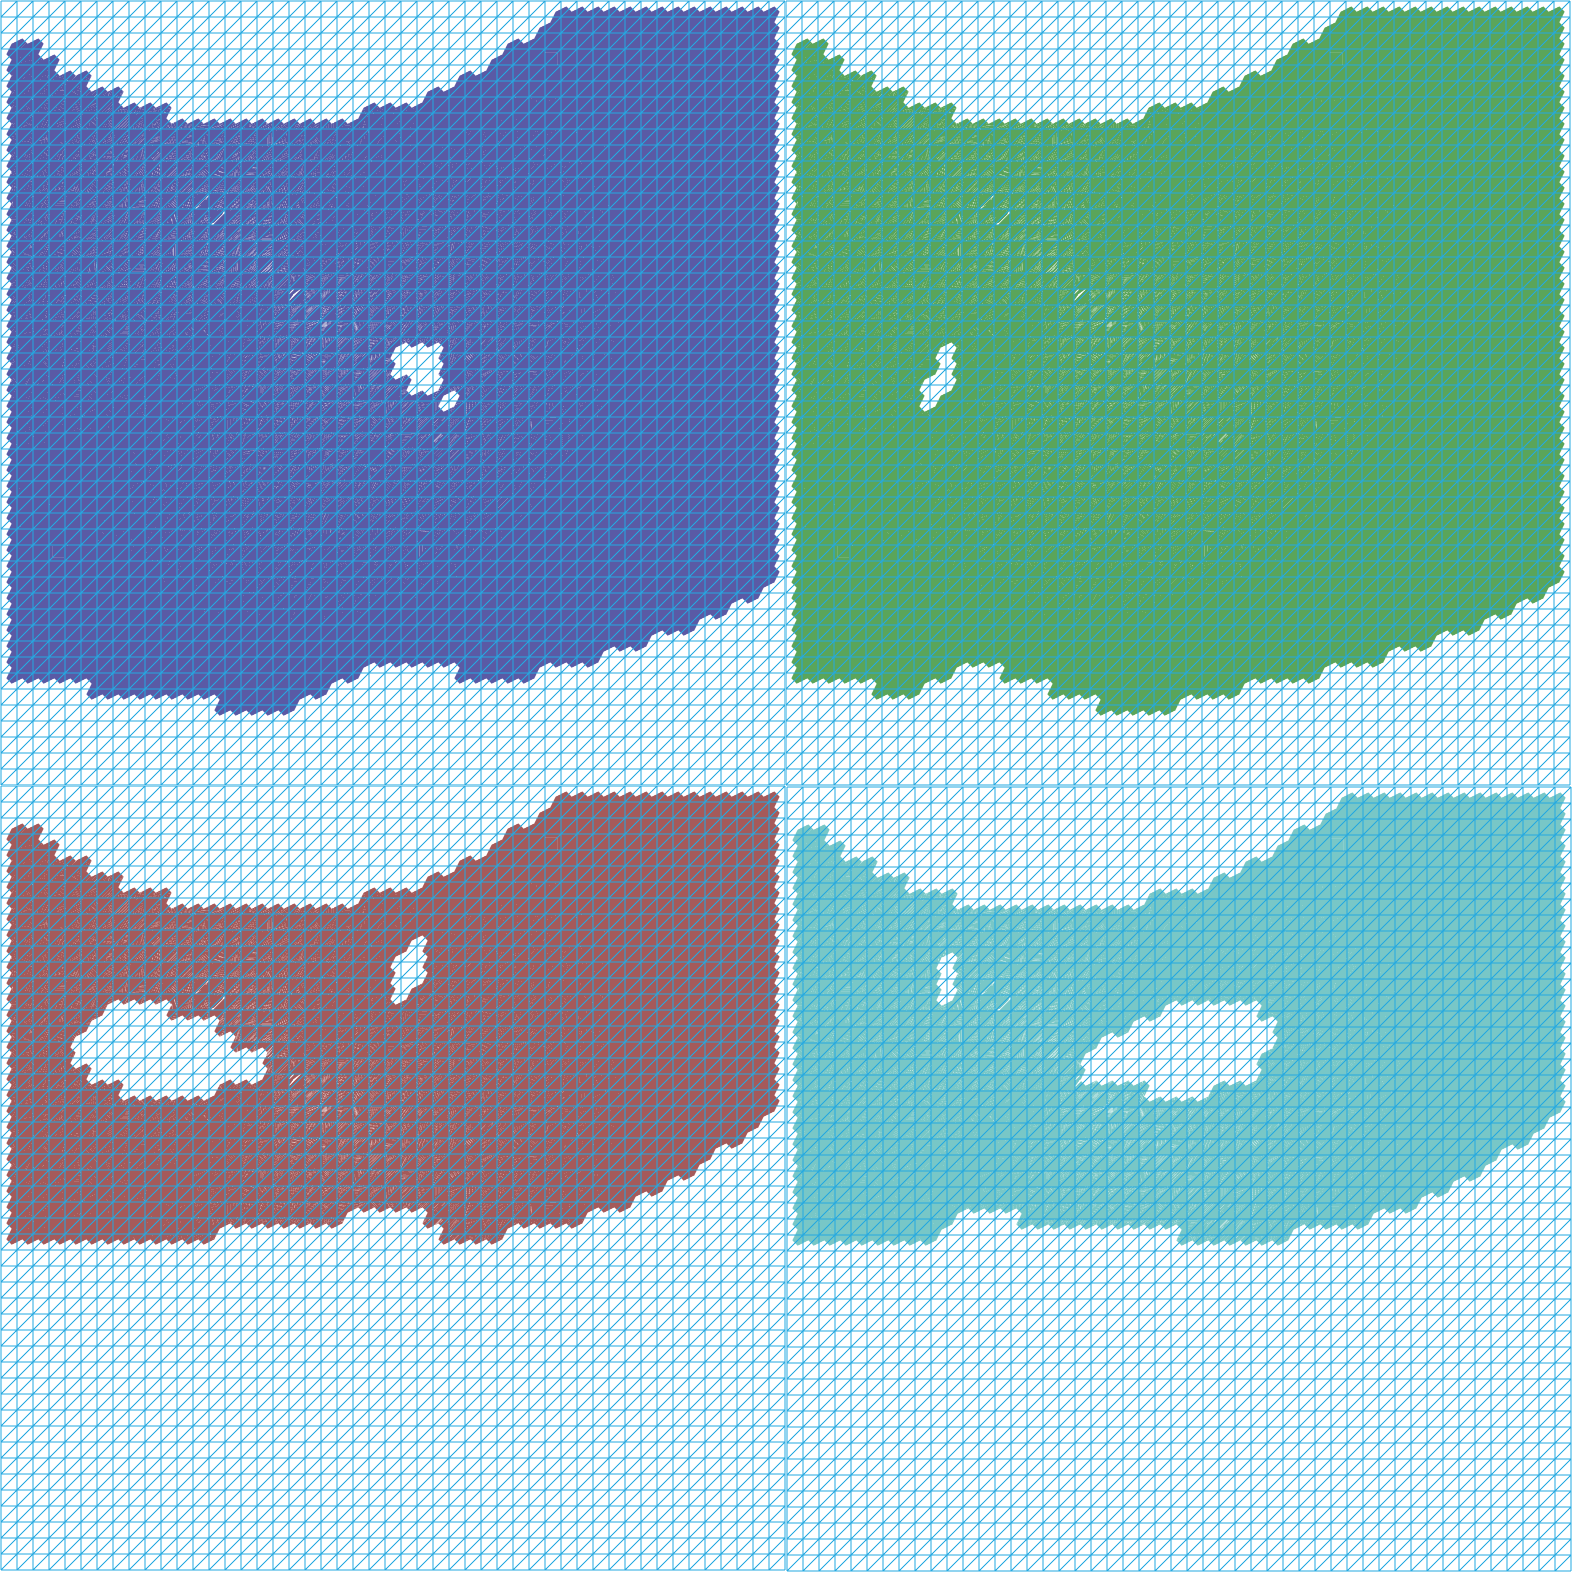
\includegraphics[width = 0.15\textwidth]{figures/hill_exp/0_06/color_comb}
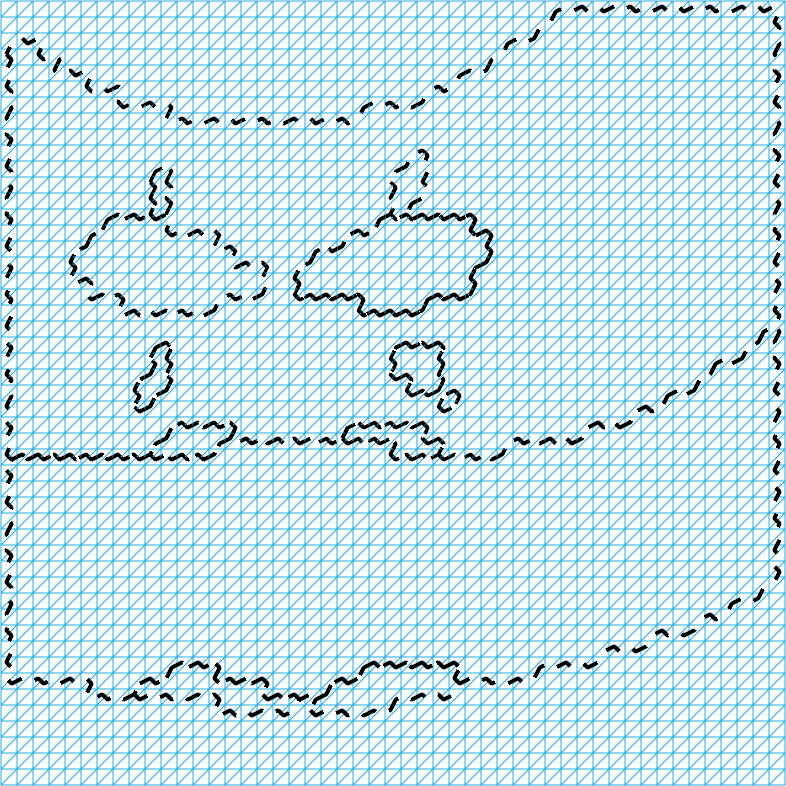
\includegraphics[width = 0.15\textwidth]{figures/hill_exp/0_06/init_graph}
}
\subfigure[Left: The color shows the manipulability of the fourth kind of configurations 
(shoulder-right, elbow-up and wrist-flipped). Middle: A configuration with relative high manipulability. 
Right: A configuration with relative low manipulability. ]{
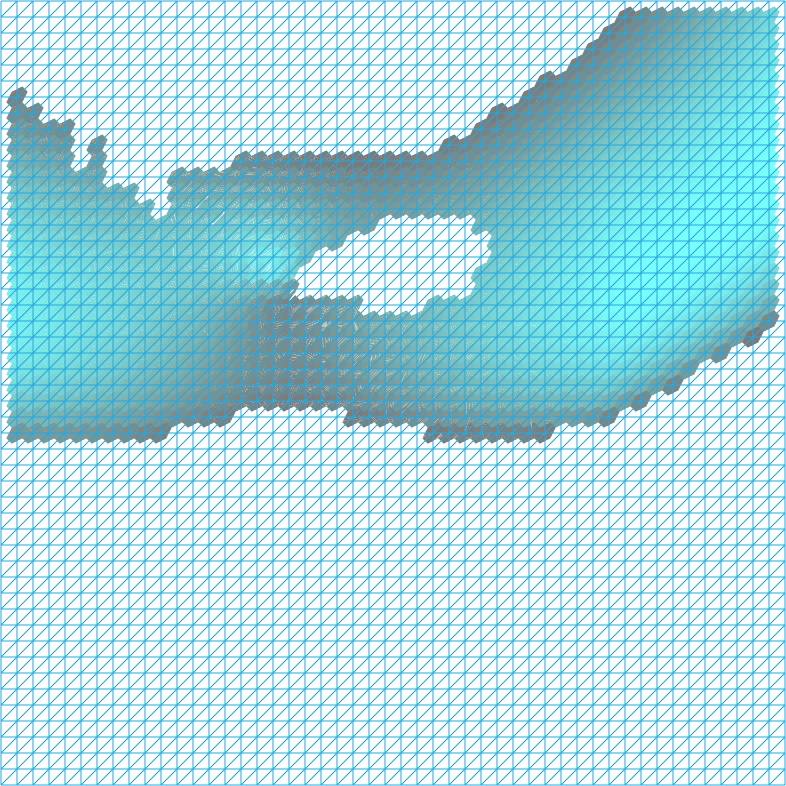
\includegraphics[width = 0.15\textwidth]{figures/hill_exp/0_06/color_4_manipulability}
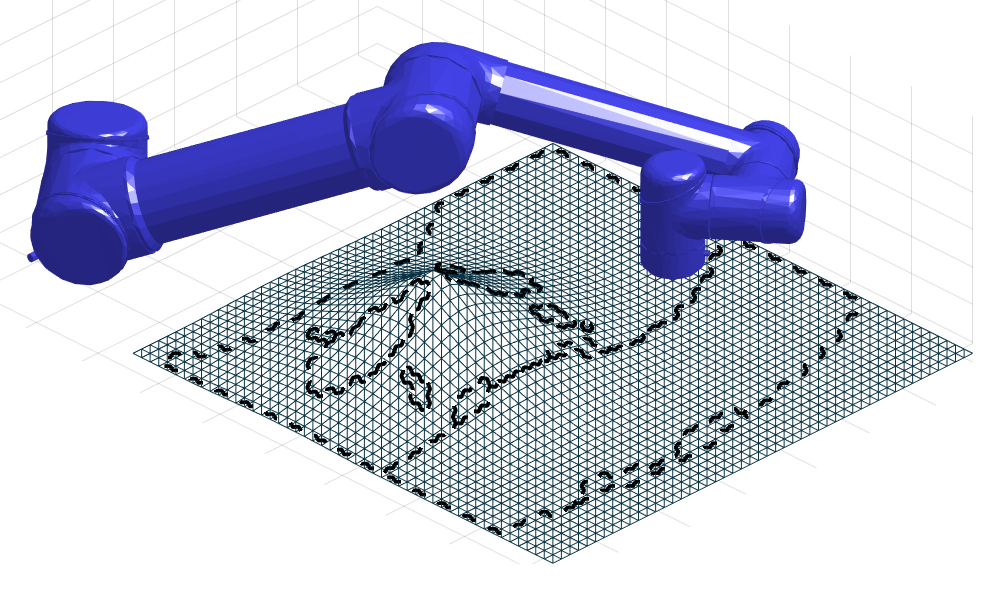
\includegraphics[width = 0.15\textwidth]{figures/hill_exp/0_06/high_manipulability_demo}
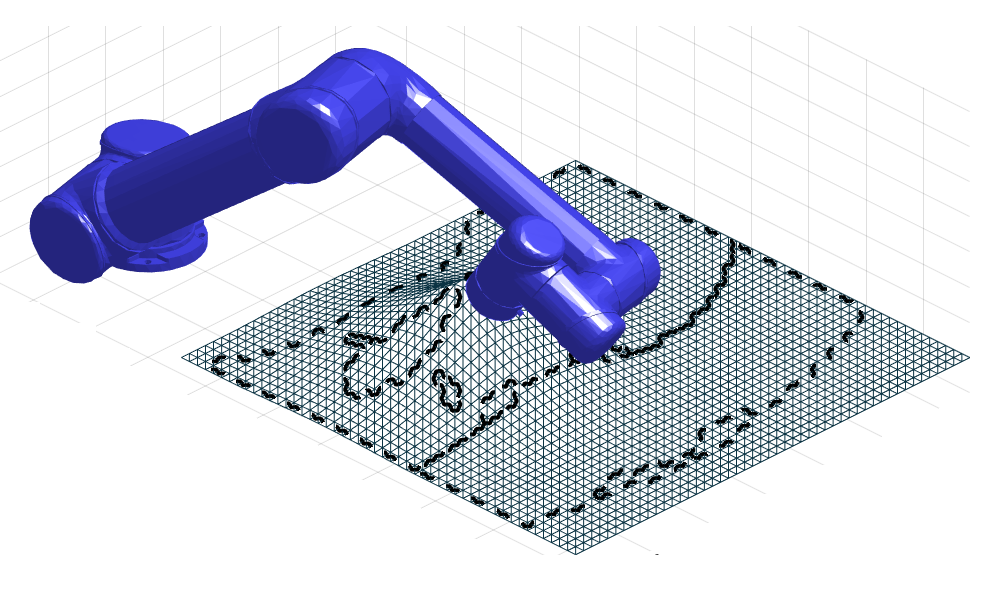
\includegraphics[width = 0.15\textwidth]{figures/hill_exp/0_06/low_manipulability_demo}
}
\caption{In (a),  examples of configurations and the topological graph are shown. The threshold of the 
manipulability is constant value. We can see the emerging of the non simply-connected cells. 
In (b), the manipulability of the configurations are visualized. If non-constant thresholds are applied, then 
more ``holes" may appear in the generated topological graph. }
\label{fig:hill_multiply_conn}
\end{figure}
\end{comment}

\begin{figure}[t]
\centering
\subfigure[]{
	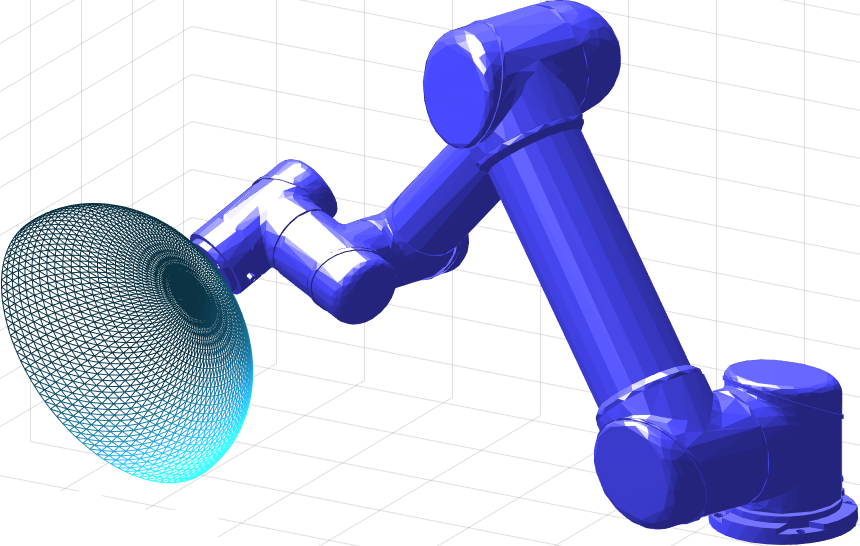
\includegraphics[width = 0.1\textwidth]{figures/TMech_simply_connected_example/design_demo_2}
	\label{fig:TMech_model}}
\subfigure[]{
	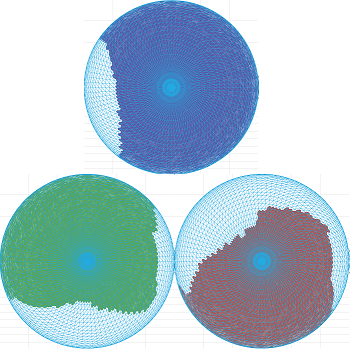
\includegraphics[width = 0.1\textwidth]{figures/TMech_simply_connected_example/design_comb}
	\label{fig:TMech_config_cells}}
\subfigure[]{
	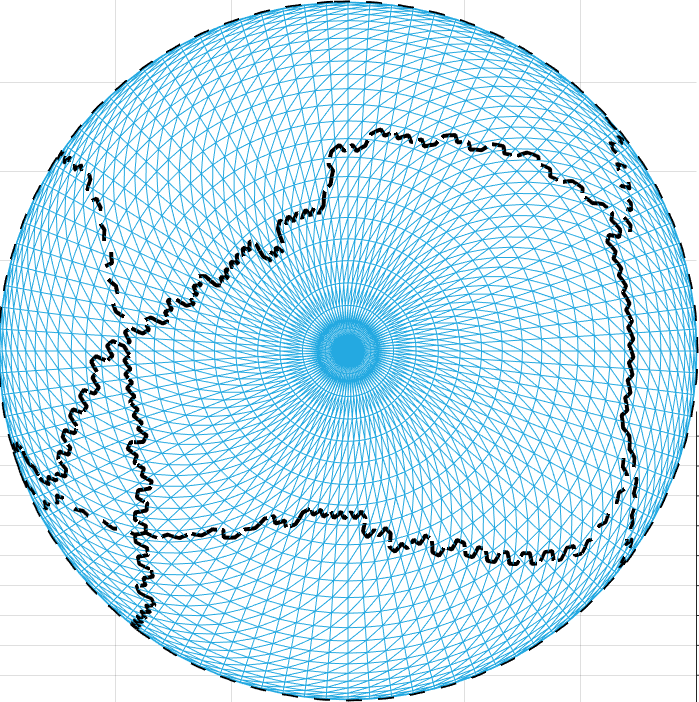
\includegraphics[width = 0.1\textwidth]{figures/TMech_simply_connected_example/design_init_graph}
	\label{fig:TMech_topo_graph}}
\subfigure[]{
	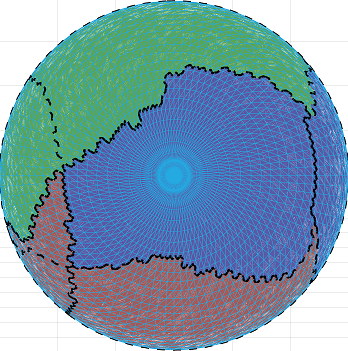
\includegraphics[width = 0.1\textwidth]{figures/TMech_simply_connected_example/design_result_graph}
	\label{fig:TMech_solution}}
\caption{Example of simply-connected cell coverage. (a) Hemispherical object placed in the workspace. 
(b) Simply-connected cells of three valid robot configurations, chosen by the optimal solution shown in (d). 
(c) Topological graph. (d) One optimal solution requiring 2 lift-offs. % and achieving full coverage. 
}\label{fig:TMech}
\end{figure}


\begin{figure}[t]
\centering
\subfigure[]{ 
	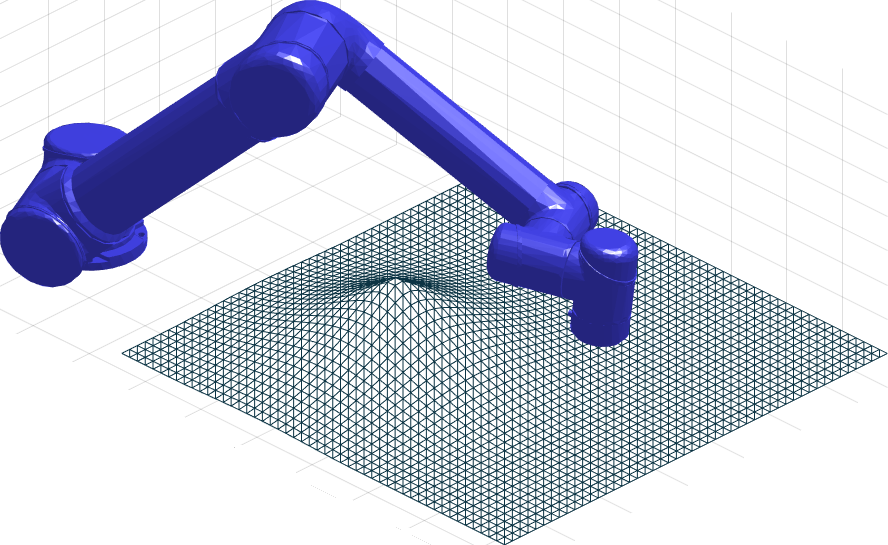
\includegraphics[width = 0.1\textwidth]{figures/hill_exp/0_06/new/demo}
	\label{fig:hill_model}}
\subfigure[]{	
	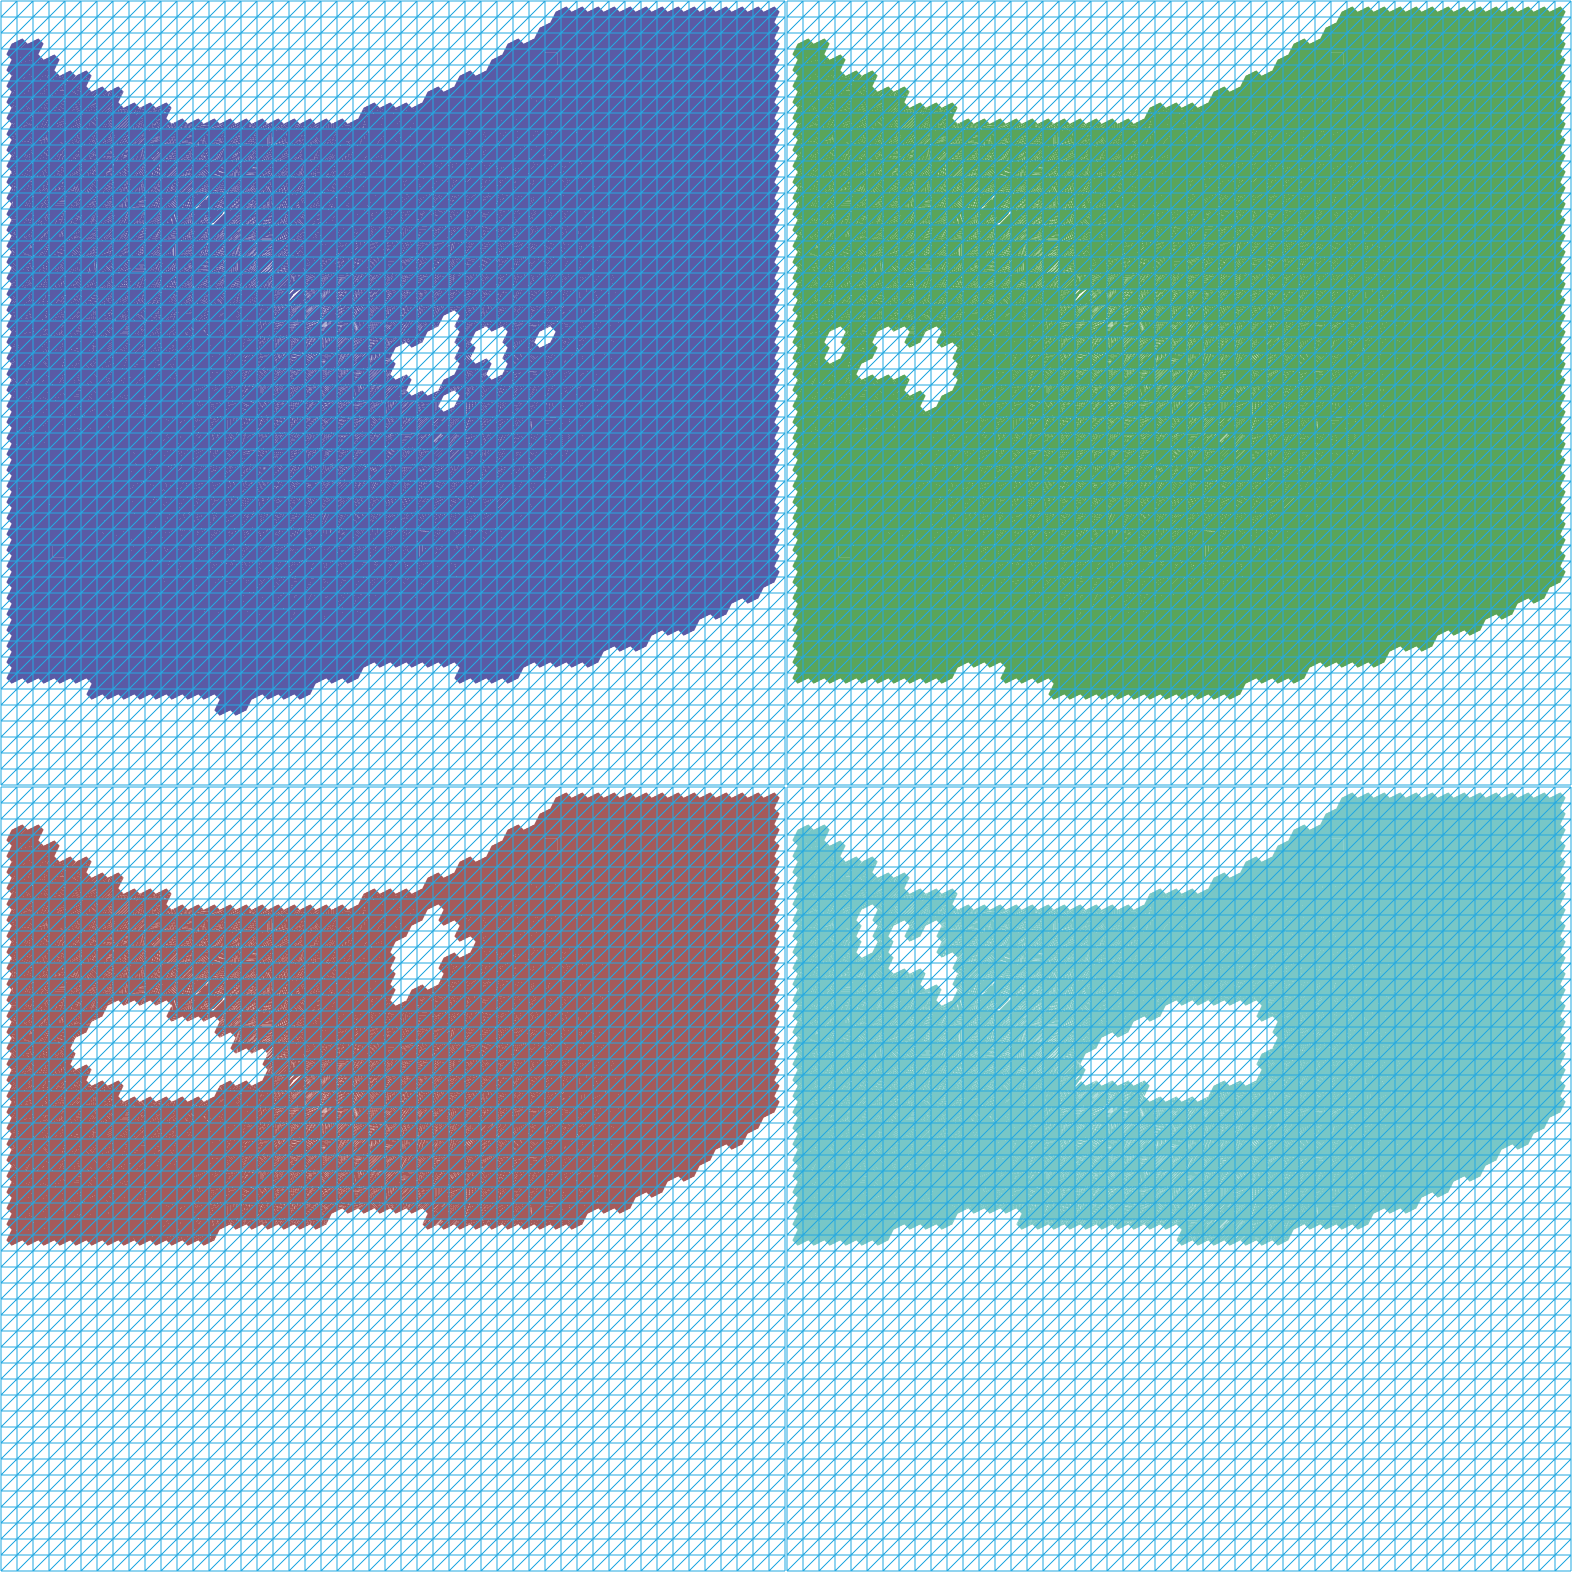
\includegraphics[width = 0.1\textwidth]{figures/hill_exp/0_06/new/color_comb}
	\label{fig:hill_config_cells}}
	\subfigure[]{	
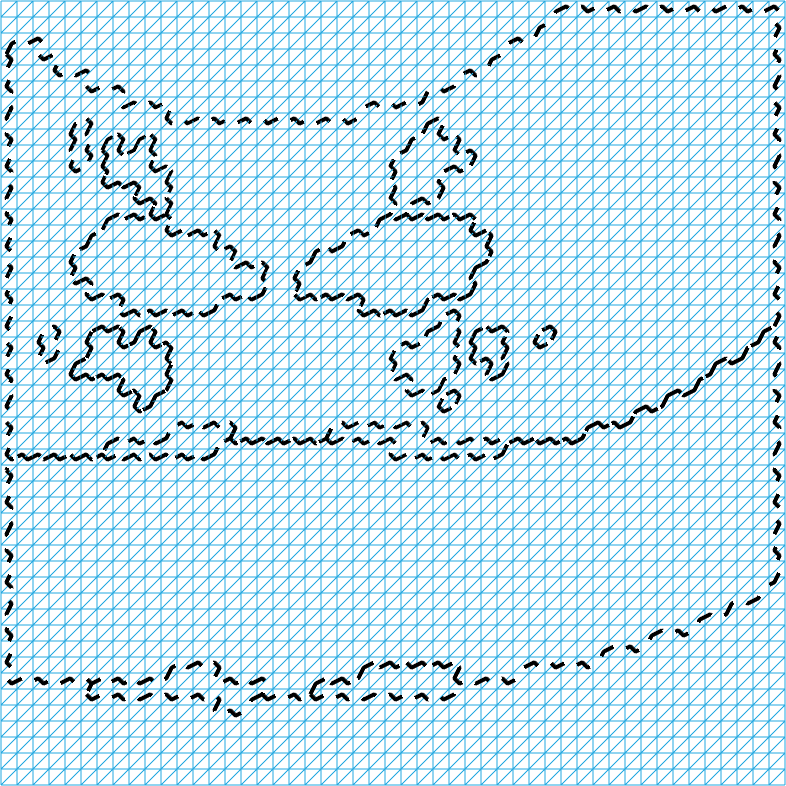
\includegraphics[width = 0.1\textwidth]{figures/hill_exp/0_06/new/init_graph}
	\label{fig:hill_config_cells}}
\subfigure[]{	
	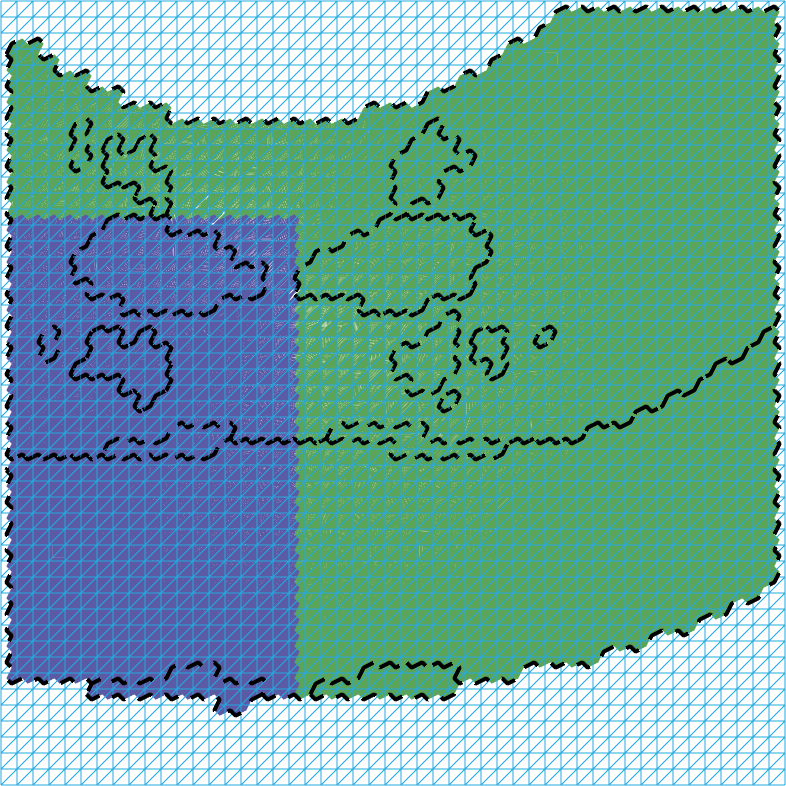
\includegraphics[width = 0.1\textwidth]{figures/hill_exp/0_06/new/result_graph}
	\label{fig:hill_solution}}
\caption{Example of multiply-connected cell coverage. (a) Irregular ``hilly'' object placed in the workspace. 
(b) Multiply-connected cells of four valid robot configurations, chosen by the optimal solution shown in (d). 
(c) Topological graph. (d) One optimal solution requiring 1 lift-off.}
\label{fig:hill_multiply_conn}
\end{figure}

A critical assumption however is that the constituent surface points necessarily adopt simply-connected space topologies. 
This is reasonable for simple shapes and sparse obstacle environments, but becomes unrealistic as objects grow in complexity, 
or with the imposition of increasing motion constraints, generically deriving in multiply-connected cells. An illustrative example is 
given in Fig.~\ref{fig:hill_multiply_conn} where a manipulator moving over a ``hilly'' terrain generates reachable areas in the
 mesh which contains non simply-connected cells. This is further compounded when additional or more restrictive constraints are imposed, 
 as will be seen later in the results when the degree of manipulability is also considered and more ``cavities'' appear in the configuration 
 cells and generated topological graphs.

%The more discontinuities of coverage path mean that lifting manipulator off the object's surface more, which lead to avoidable complexity of transiting between position and force/torque control.
%In our previous work, the optimal coverage path planning problem ensuring minimum discontinuities is formulated as a painting scheme for a graph ensuring least discontinuities. 
%However, possibly because the constraints given in our previous work are simple (only kinematic, static force and manipulability are considered, and the thresholds are constant value), all cells are in simply-connected case. 
%And our proof of the finiteness of divisions only works for simply-connected cells which only contains one boundary. Although it is applicable for most physical cases, it is theoretically incomplete. Hence, our aim in this paper is to present a general proof of the finitness of solving all topological graphs, and present an iterative solver. 

Since the shape of cells can be classified through their genus, i.e., the number of ``holes" within the cell, in this work a 
theoretically complete solution is given by solving for cells with all possible genus. The key observation of the proposed algorithm is that 
whatever genus the cell is, the number of lift-off to cover it is always zero. % <jvm> this the same as saying it is equivalent to our TMech approach, when each simply-connected cell also has zero lift-off. Contrbution is how to transform the problem to get there
A direct reflection from this is thus to reduce the genus of the cell gradually by cell divisions to eventually make it equivalent to a 
simply-connected cell which has been proven finitely solvable. This however is non-trivial: the place to put a cutting path to transform 
a genus-one cell into a simply-connected cell directly effects the order of edges on the boundary of the sub-cells, leading to different structures. %So the division process is not trivial.  
Existing algorithms in the literature are not able to provide a systematic cell decomposition solution to accomplish a guaranteed 
transformation from an initial graph containing large genus cells into simply connected topologies. This is provided in this work through 
the analysis of equivalent topological divisions. To that extent, the finiteness of all possible divisions is first proven for a genus-one cell as 
building block. A multi-stage iterative solver can then be introduced to transform higher-genus cells into lower-genus cells. The two novel 
contributions of this paper can be thus summarised as:
\begin{enumerate}
\item Providing the necessary conditions to be able to apply the surface modeling described by the proposed topological graph structure. %Fixed <jvm> Tong pls check above sentence is correct in your view, I changed txt, need to be sure it remains correct %<ty> Yes, it is true. The contribution is given in section 4
\item Proposing a systematic solution to be applicable for any genus-$n$ cell topology. 
\end{enumerate}

The remainder of this paper~\footnote{A video illustrating the concepts hereby described can be found 
here:\url{https://youtu.be/TqFzqGGM06Y}} is organised as follows. 
Section~\ref{section_related_works} reviews existing literature. 
Section~\ref{section_finiteness_of_cells} proves the necessary conditions to apply the proposed algorithm. 
Section~\ref{section_simply_connected} briefly restates the existing results in~\cite{Yang2020Cellular} to solve for 
simply-connected cells. Section~\ref{section_genus_one} goes into further details about the finiteness of solving elementary genus-one cells, whilst 
a multi-stage iterative strategy to solve for larger genus-$n$ cells is described in Section~\ref{section_large_genus}. 
Experimental results from simulations are collected in Section~\ref{section_exp}, with final concluding remarks gathered in 
Section~\ref{section_conclusion}.

\section{Related Works}\label{section_related_works}
Almost all state-of-the-art methods to solve the coverage path planning (CPP) problem~\cite{choset2001coverage}~\cite{galceran2013a} 
first divide the target surface into cells then solve the CPP problem in each cell, so called cellular decomposition, which is further divided 
into two categories: exact cellular decomposition methods~\cite{lumelsky1990dynamic} and Morse-based cellular decomposition 
methods~\cite{choset2000exact}~\cite{Acar2002Morse}. 

%For the coverage task of the manipulator, 
%~\cite{rososhansky2011coverage} considered the contact mechanics problem to solve the tool-path planning problem. 

For the optimal coverage task with a manipulator, the algorithms mainly focus on workspace metrics such as path length and time to completion. 
Atkar \textit{et al.}~\cite{Atkar2003Towards} optimised the coverage path through choosing optimal starting points. 
Huang~\cite{huang2001optimal} reduced movement cost by remaining on straight paths as long as possible thus minimising the number of turns.
In dealing with the optimal Non-revisiting Coverage Path Planning (NCPP) problem,~\cite{Atkar2008Hierarchical} considered 
the uniform coverage in automotive spray painting problem, where the simple back-and-force boustrophedon path was deformed in accordance 
to the curvature and topology of the surface.~\cite{hameed2016side-to-side} proposed a 3D coverage path for agricultural robots 
minimising the skip/overlap areas between swaths. 

Its is arguable however that for surface contact tasks in particular, the cost incurred in joint discontinuities significantly 
outweighs other metrics, moreover where undesirable transitions between position and force/torque control~\cite{cheah2003brief}~\cite{heck2015switched}~\cite{mirrazavi2018a}~\cite{solanes2018adaptive}~\cite{Solanes2018Robust} become unavoidable. %~\cite{cheah2003brief}~\cite{heck2015switched} 

%In dealing with the optimal non-revisiting coverage path planning (NCPP) problem, the mainstream discussions on the non-revisiting property focus only in the microlevel, i.e., the physical place of the coverage path. For example,~\cite{Atkar2008Hierarchical} considered the uniform coverage in automotive spray painting problem, where the simple back-and-force boustrophedon path are deformed based on the curvature and the topology of the surface.~\cite{hameed2016side-to-side} proposed a 3D coverage path for agricultural robots minimising the skip/overlap areas between swaths. 

% <ty> Should we still mention Paus's work if we don't mention "optimal placement"? 
We notice that~\cite{paus2017a} considered the pose optimisation of a mobile manipulator for coverage task, 
where a quality measurement was proposed to optimally place the manipulator in the workspace to aid coverage. 
The focus remained complementing robot placement and CPP; the actual generation of the coverage path simply reduced to use 
a randomised path planner, BiRRT~\cite{LaValle2001Randomized} % <jvm> Tong what is BiRRT? I guess an RRT, hence randomised, correct otherwise
among a set of  ``guard points" chosen, with no specfic consideration to joint-space continuity as ellaborated in the present manuscript. 
%And their work is not applicable for NCPP problem. 

It is worthwhile noting that despite the apparent similarities in planning with mobile platforms, the optimal NCPP problem with least discontinuities 
is inherent to the kinematics of manipulator mechanisms, and as such beyond the scope of bibliograpic works from the mobile robotics community.
%s will not encounter such problem. 
Likewise, affinities to graph theory are also legit. Note however that the contact point, which can be safely regarded as a particle, 
is significantly smaller than the scale of the cellular decomposition drawn up for this problem. 
In seeking maximal joint-space continuity of the coverage path travelled by a particle as modelled by the NCPP problem, 
infinitesimal elements must be considered in its most abstract form, and the existance of infinitely narrow passages also 
makes a significant difference in the resulting path solutions. % (potentially much larger than the contact point) 
% <jvm> Tong I don't fully understand what you have written still. But if what I say, derived from you rwritting, is correct and make sense to you, pls leave, or modify VERY BRIEFLY. I really want you to explain this to me, but separately. I would like to see an illustration of this in the video for instance.
Hence, it is not possible to revert back to classical graph theory since no any area on the surface can be seen as a whole to form the "vertices", 
and the set of "edges" is actualy the exact solution the NCPP problem is seeking to solve for. 


\section{Problem Statement}
Define the surface of an object by $M$. To simplify the description, let $M$ be only the coverable part of the surface. 
The shape of other obstacles in the workspace and their relative poses in the workcell are assumed static and known.
%The boundaries of $\Omega$ and $M$ are denoted by $\{\partial \Omega_i\}_{i\in \mathbb{N}}$ and $\{\partial M_i\}_{i\in \mathbb{N}}$, respectively. 
Given the kinematics of the non-redundant manipulator, we denote the joint-space by $\bar{\mathscr{C}}$, and the set of all singular configurations by $S$. 
The set of all valid manipulator configurations is denoted by $\mathscr{C}$, where the validity of a configuration is evaluated by some given quality constraints denoted by $\{F_k\}_{k\in \mathbb{N}}$. Classic examples would be manipulability or the minimum distance from an obstacle. 
%(Non-singularity is not enough for validity, and the differences between $\mathscr{C}$ and $\bar{\mathscr{C}}\backslash S$ will be shown below). 
%The shape of other obstacles in the workspace and their relative poses to the manipulator are totally known. 
%Some quality measurements and their threshold (e.g. the manipulability introduced by~\cite{}) are also given. 
The optimal CPP problem is to find a joint-space path consisting of valid configurations whereby the manipulator EE covers the workspace non-repetitively 
and ensures the least number of discontinuities requiring lifting from the object's surface. The following settings define the scope formally: 
\begin{enumerate}
%\item The $\{\partial\Omega_i\}$ should be well-defined. For example, to make the normal vectors of a boundary point $m\in \{\partial \Omega_i\}$ meaningful, $m$ should be an inner point of the surface $M$. In other words, 
%\begin{equation}
%\partial \Omega_i\subset M\backslash \left(\bigcup\limits_{j} \partial M_j\right), \forall i
%\end{equation}
\item A point contact between surface and EE is assumed. 
\item 
\begin{comment}
%Fixed <jvm> Tong, commented this out, I don't see it is required, it is obvious singularities are out of our search space, save some space. IFF you feel it mathematically necessary for completeness, reintroduce. 
% <ty> I think it depends on how the robotists see the coverage task using the manipulator. If all people think the same as you, then we can safely comment this. And I believe the reviewers think the same as you. 
The singular configurations $S$ and their neighbours are beyond the scope of our discussion even if the manipulability constraint is not explicitly considered, i.e., 
\begin{equation}
\mathscr{C}\subset \bar{\mathscr{C}}\backslash S
\end{equation}
To quantify the relation, 
\end{comment}
Let $s\in S$ be a singular configuration, there exist a threshold $\epsilon > 0$ such that 
\begin{equation}
d(c, s) > \epsilon, \forall c\in \mathscr{C}, \forall s\in S
\end{equation}
where $d(\cdot, \cdot)$ is a metric in the joint-space. This enables us to judge the discontinuity of two configurations coming from discretised data. 
For example, given two configurations $c_1, c_2\in \mathscr{C}$ corresponding to the EE covering two adjacent vertices of a triangular mesh, we say $c_1$ and $c_2$ are joint-space continuous only if 
\begin{equation}
%c_1 \mbox{ and } c_2 \mbox{ are continuous}\Leftrightarrow 
d(c_1, c_2) < \epsilon
\end{equation}
where $d(\cdot, \cdot)$ and $\epsilon$ are pre-determined. 
\item $\{F_k\}_{k\in \mathbb{N}}$ is continuously defined in the joint-space, with thresholds satisfying strict inequalities. 
The $k$-th constraint can be expressed as
\begin{equation}\label{equ_strict}
F_k(c) > \delta_k = \delta_k(c, F_1, \cdots, \hat{F}_k, \cdots, F_{n}), \forall c\in \mathscr{C}
\end{equation} 
where ``$\hat{\ }$" means excluding the term. $\delta_k$ can be a function of other metrics instead of a constant value, leading to wider applications. 
For example, let $F_1$ represent the manipulability~\cite{yoshikawa1990translational} 
and $F_2$ represent the minimum distance between the manipulator and all obstacles, then an inequality such as
$$
F_2(c) > \delta_2 = 0.01+0.05(1-F_1(c))
$$
could be imposed to indicate that when $F_1(c)$ is small, i.e. a ``badly-conditioned" configuration, it should be farther from obstacles than would be desirable otherwise. 

\end{enumerate}
\section{Finiteness of Cells}\label{section_finiteness_of_cells}
\begin{comment}
%Fixed <jvm> Tong, I don't understand why this is here when we are restricted to discuss the finitness of the graph. I feel unncessary hence commented out. 
% <ty> Yes, you are true. The function of this sentence is only to note myself not forgetting introducing the modelling process if necessary. So does some later sentences in red. 
\begin{color}{red}
The process of transforming the optimal CPP problem into optimal painting problem is omitted here. 
\end{color}
\end{comment}

%First, we give the definitions for the elements in our algorithm. 
For a non-redundant manipulator, $\forall m\in M$ there exist a finite number of valid configurations to cover $m$. 
By following the constraints laid out in the problem statement, a topological graph will be generated. 
A necessary condition to solve it is thus guaranteeing the finitness in the number of cells on this graph. For that, let us define a topological 
cell $C_1$ (where $1$ represents its index) as a maximal set of continuous points where the valid configurations to cover them are 
pairwise continuous, i.e., $\forall m, m'\in C_1$, let the valid configurations to cover them be 
\begin{equation}\label{equ_pm}
P_{m} = \{c_{m1}, \cdots, c_{mN}\}\subset \mathscr{C}
\end{equation}
\begin{equation}
P_{m'} = \{c_{m'1}, \cdots, c_{m'N'}\}\subset \mathscr{C}
\end{equation}
then $N = N'$ and
\begin{comment}
\begin{equation}
\begin{aligned}
 \forall c_{mi}\in P_m, &\exists c_{m'j}\in P_{m'},& 
&c_{mi} \mbox{ and } c_{m'j}  \mbox{ are joint-space continuous}
\end{aligned}
\end{equation}
\end{comment}
$\forall c_{mi}\in P_m, \exists c_{m'j} \in P_{m'}, c_{mi}$ and $ c_{m'j}$ are joint-space continuous.

A topological edge $E_1$ (where $1$ represents its index) is a maximal set of continuous points  between $C_i$ and $C_j$ whereby
%\begin{equation}
\begin{flalign}
 E_1 & =   \, E_1(C_i, C_j) \nonumber \\
       & =  \left\{m\in M| \forall (m\in )U_m, \exists p, p'\in U_m, p\in C_i, p'\in C_j\right\}
\end{flalign}
%\end{equation}
where $U_m$ is an open set containing $m$. 
Note that the intersecting points of topological edges 
\begin{equation}
\{m| \forall (m\in )U_m, \exists p, p', p''\in U_m, p\in C_i, p'\in C_j, p''\in C_k\}
\end{equation}
are distinct points, which is negligible when discussing the connectivity of the cells. 
The topological graph is the ordered cells and edges, $G = (\{C_i\}, \{E_j\})$. 

To prove the finitness of this graph, let us randomly choose a point $m\in M$ which can be covered by a set of valid 
configurations $P_m$ defined by (\ref{equ_pm}), then 
\begin{equation}
F_k(c_{mi}) > \delta_{k}, \forall k, \forall i = 1, \cdots, N
\end{equation}
the strict inequalities (\ref{equ_strict}) enable us to find valid open sets $U_{mi}$ for each configuration $c_{mi}$ in the joint-space:
\begin{equation}
\begin{aligned}
&\exists (c_{mi}\in )U_{mi} \subset \mathscr{C}, \forall i = 1, \cdots, N \\
\mbox{s.t.}\mbox{  } F_k(c) > \delta_k + &\frac{1}{2}(F_k(c_{mi}) - \delta_k)> \delta_k, \forall k, \forall c\in U_{mi}
\end{aligned}
\end{equation}
since the kinematic function of the manipulator (${\rm FK}$) is continuous and $c_{mi}\in U_{mi}$, 
\begin{equation}
m\in {\rm FK}(U_{mi})\subset M, \forall i = 1, \cdots, N
\end{equation}
so does the intersecting area of those images, 
\begin{equation}
m\in A_m \triangleq\bigcap\limits_{i = 1}^N\left({\rm FK} (U_{mi})\right)\subset M, \forall i = 1, \cdots, N
\end{equation}
follow the definition of our topological cells, all points within the intersecting area belong to a same cell. 

For $\forall m\in M$, the corresponding open set $A_m$ exists, as such %Apparently
\begin{equation}
\bigcup\limits_{m\in M}A_m\supseteq M
\end{equation}
hence the left term forms a infinite cover of $M$. %Following the Heine-Borel Theorem~\cite{} % <jvm> Tong pls add % <ty> I will try. 
%It is one of the most fundamental theorems in mathematical analysis (like the inverse kinematic function in manipulator area. ) so possibly no original publication can be found.  
The Heine-Borel Theorem~\cite{Simmons1964Introduction} states that if a compact region can be covered by infinite many open regions, then one can find finite many of them that still fully cover this region. Since all closed sets in the Euclidean space are compact sets, so is the manipulator 
task space in which the boundaries are well-defined. Thus, we can find finite elements from $\{A_m\}_{m\in M}$ that also fully 
cover $M$. Recall that each $A_m$ belongs to only one cell, hence the total number of cells in the graph must be finite.  

%\begin{figure}[t]
%\centering
%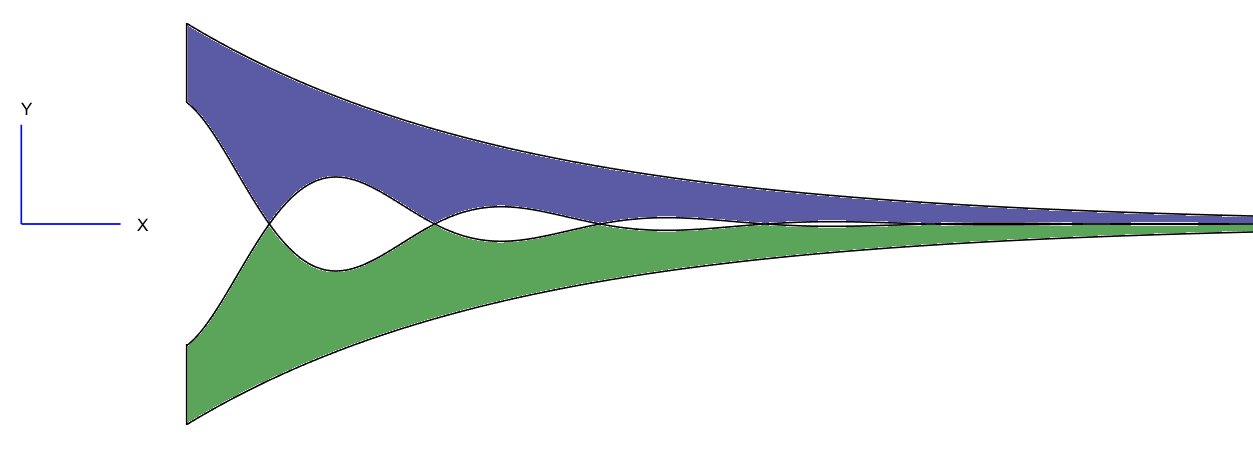
\includegraphics[width = 0.4\textwidth]{figures/proof/fig_counterexample}
%\caption{This figure gives a counter-example that the intersection two finite-area regions is the disjoint union of infinite many regions. The equations of the boundary for the blue colour is $y_1 = e^{-x}$, $y_2 = e^{-2x}\cos(2\pi x)$, $x = 0.5$. And the green region is symmetric about the $x$-axis. For each $k\in \mathbb{N}$, when $x\in (k-\frac{1}{2}, k+\frac{1}{2})$, a simply-connected intersection is created, so the components of the intersection of two colours is infinite. }\label{fig_counterexample}
%\end{figure}


\section{Solving Graphs with Simply-Connected Cells}
\label{section_simply_connected}
In earlier work~\cite{Yang2020Cellular}, the optimal NCPP problem with least discontinuities was also modelled as a 
topological cell graph, and the solution transformed into an optimal design strategy of a colour (configuration) scheme whereby the strategic placement of cutting paths would invariably 
lead to different colour vertices on both sides of a partition. An illustrative example is provided by Fig~\ref{fig:TMech}. 
In proving the finiteness of simply-connected cells, the following claims were validated:
\begin{enumerate}
\item It is sufficient to consider cutting paths that start and end at the topological edge end-points. 
\item It is unnecessary to consider cutting paths that stretch across edges.
\item Intersecting cutting paths can be discarded. 
\item For a simply-connected cell with $K$ topological edges delineating its boundary, a binary number of length $K$ 
can uniquely specify the set of all admitted divisions. 
\item To solve a simply-connected cell with $K$ edges, the total number of different divisions $\Phi$  is bound by %$\Phi(K) \leq 2^K$. 
% <jvm> Tong check pls 
\begin{equation}
\label{equ_Psi}
\Phi(K) \leq 2^K
\end{equation}
\end{enumerate}
%where $\Psi$ and $\Phi$ are both defined for later consistency.  
In the following sections, a generalisation to genus-$n$ cells is derived.

\section{Solution of Genus-One Cells}
\label{section_genus_one}
A cutting path connecting the inner part and the outer part of a genus-one cell will transform the cell into a 
simply-connected cell, % <jvm> Tong I know you find this trivial, but this sentence is crying for a ref.! see if you can find one pls
% <ty> keep searching. Possibly end up with a book of point-set topology
proven to be finitely solvable. 
In this section we consider two cases: keeping the genus-one structure or transforming the genus-one cell into 
simply-connected sub-cells. In the former case, we prove that the inner part and the outer part can be seen as two independent problems. 
While in the later case, by efficiently discarding equivalent cellular decompositions, the number of possible subdivisions is proven to be finite, 
and all optimal solutions thus finitely solvable. An upper-bound on the complexity of solving a genus-one cell is also derived.  

For notation, a genus-one cell is denoted by $\Omega$, with its inner boundary and outer boundary denoted by $\omega$ and $\omega'$, 
respectively. The edges and cutting paths are denoted by $\alpha$. 

\subsection{Independence of Inner and Outer Parts}
\label{subsection_un_inner_cell}
\begin{figure}[t]
\centering
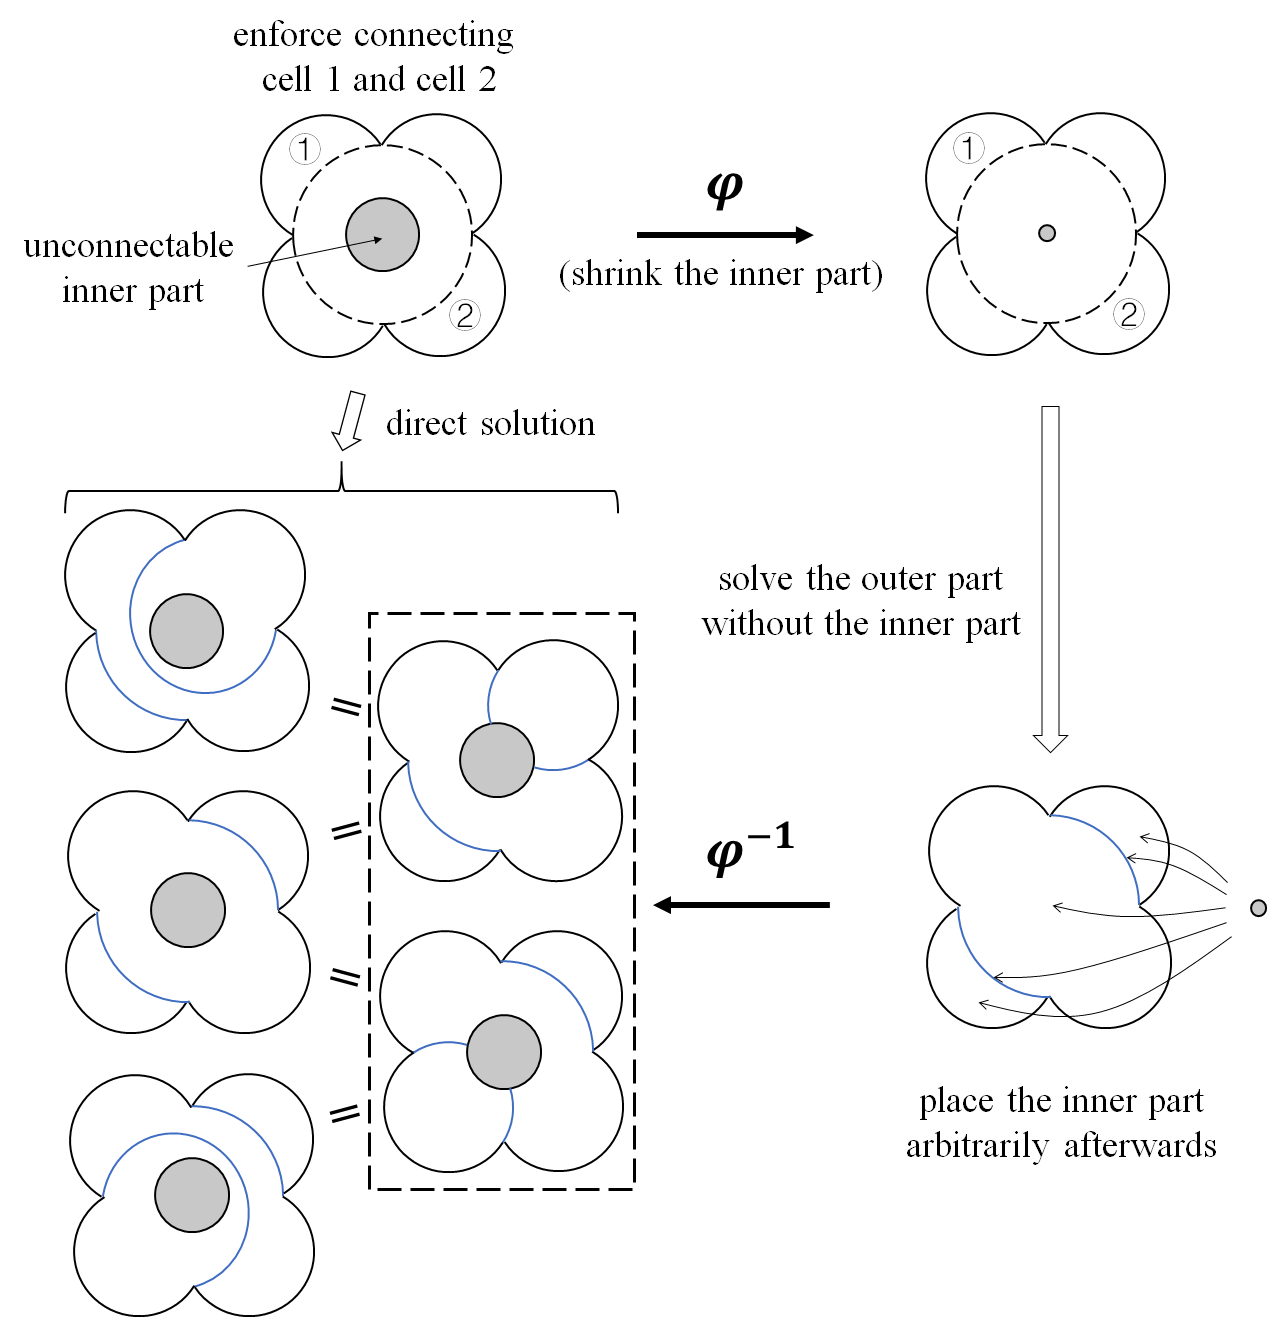
\includegraphics[width = 0.44\textwidth]{figures/proof/fig_physical_hole_5}
\caption{Example showing that the unconnectable inner part (marked by the grey solid circle) is negligible when solving the outer part. 
$\omega$ and $\omega'$ are directly drawn as concentric circles so $\varphi(\omega') = \omega'$. 
In this simple example the direct solutions are straightforward, and they are equivalent to first solving the outer part without the inner part, 
and then arbitrarily replacing back the inner part. It can also be observed how the inner part can be placed ``on'' a cutting path 
(dashed block), yet there is no need not consider these cases since they are effectively equivalent to the three divisions shown on the left under 
a continuous cutting path transformation.}
 \label{fig_physical_hole}
\end{figure}

The situation when inner part and the outer part of $\Omega$ are not connected arises when the inner part is a physical hole, 
the inner part can only be covered with a totally different colour from that of the outer part, or when all the edges in $\omega$ must be retained. 
In these cases, first we prove that the inner part of $\Omega$ is negligible when solving the outer part. 
To show this equivalence, let $\varphi$ be a homeomorphic mapping 
from $\Omega$ to the standard unit disk $D$, with its boundaries mapped onto concentric circles, 
\begin{equation}
\varphi: \Omega\rightarrow D, \omega'\mapsto S^1(1), \omega\mapsto S^1(\delta), \delta\rightarrow 0^+
\end{equation}
then the inner part becomes an infinitesimal open neighbourhood of the origin. See Fig.~\ref{fig_physical_hole} for illustration. 
Let a cutting path of $D$, $\varphi(\alpha)$, start and end at $\varphi(\omega')$, then it must be one of the following two cases:
\begin{equation}
\label{equ_nocross}
\begin{aligned}
&(0, 0)\notin \varphi(\alpha)\\
\Rightarrow &\exists \epsilon > 0, B(0, \epsilon) \cap \varphi(\alpha) = \varnothing\\
\Rightarrow &\mbox{let } \delta < \epsilon, \mbox{ then } \varphi(\omega)\cap \varphi(\alpha) = \varnothing\\
\Rightarrow & \omega\cap \alpha = \varnothing
\end{aligned}
\end{equation}
or 
\begin{equation}
\label{equ_cross}
\begin{aligned}
&(0, 0)\in \varphi(\alpha)\\
\Rightarrow &\varphi(\omega)\cap \varphi(\alpha) \neq \varnothing, \forall \delta\\
\Rightarrow & \omega\cap \alpha \neq \varnothing
\end{aligned}
\end{equation}

%\begin{align}
%&\begin{aligned}\label{equ_nocross}
%&(0, 0)\notin \varphi(\alpha)\\
%\Rightarrow &\exists \epsilon > 0, B(0, \epsilon) \cap \varphi(\alpha) = \varnothing\\
%\Rightarrow &\mbox{let } \delta < \epsilon, \mbox{ then } \varphi(\omega)\cap \varphi(\alpha) = \varnothing\\
%\Rightarrow & \omega\cap \alpha = \varnothing
%\end{aligned}\\
%\mbox{or}\nonumber\\
%&\begin{aligned}\label{equ_cross}
%&(0, 0)\in \varphi(\alpha)\\
%\Rightarrow &\varphi(\omega)\cap \varphi(\alpha) \neq \varnothing, \forall \delta\\
%\Rightarrow & \omega\cap \alpha \neq \varnothing
%\end{aligned}
%\end{align}

All the different topological divisions described by ~(\ref{equ_nocross}) and~(\ref{equ_cross}) correspond to those listed in Fig.~\ref{fig_physical_hole}.
 
Next, we prove the inverse claim that the outer part of $\Omega$ is negligible when solving the inner part.  
Let a sphere with radius $r$ stand within the inner part (anywhere is applicable but a place within the inner part will simplify the
 description), and $\psi$ be the stereographic projection%~\cite{coxeter1969introduction} % <jvm> Tong add citation. Why this projection (in one VERY short sentence, as per H-B example, to describe why we are doing this. Not clear to me. 
\begin{equation}
\begin{aligned}
\psi: \mathbb{R}^2&\rightarrow S^2\backslash N\\
(x, y, 0)&\mapsto (\frac{4r^2x}{x^2 + y^2 + 4r^2}, \frac{4r^2y}{x^2 + y^2 + 4r^2}, \frac{2r(x^2 + y^2)}{x^2 + y^2 + 4r^2})
\end{aligned}
\end{equation}
\begin{figure}[t]
\centering
\subfigure[]{ 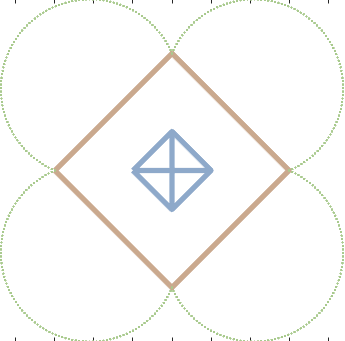
\includegraphics[width = 0.11\textwidth]{figures/proof/fig_stereo_1}}
\subfigure[]{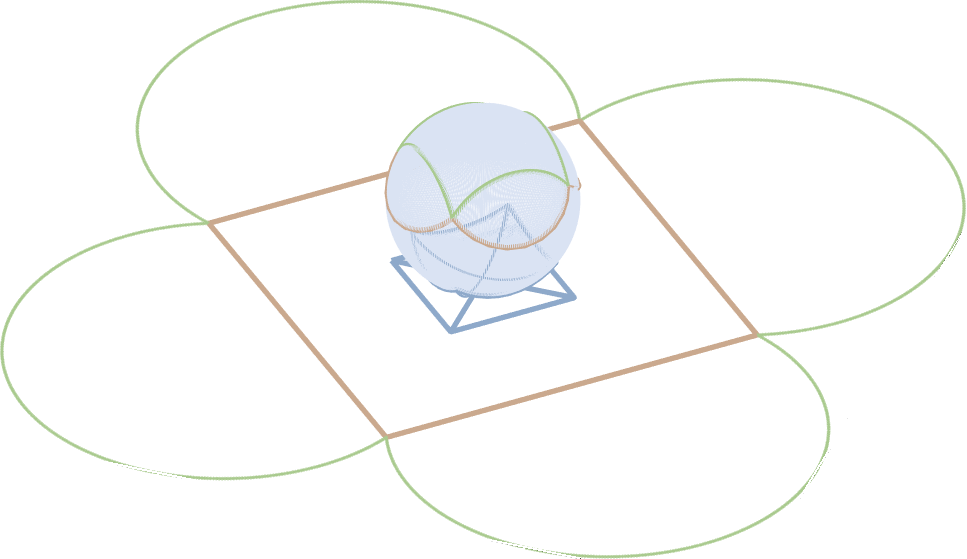
\includegraphics[width = 0.13\textwidth]{figures/proof/fig_stereo_2}}
\subfigure[]{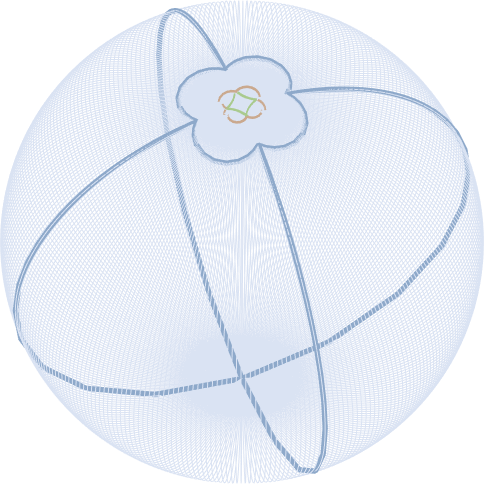
\includegraphics[width = 0.11\textwidth]{figures/proof/fig_stereo_3}}
\caption{ (a) Topological graph with a genus-one cell enforced to be kept (the area between concentric squares). 
(b) A stereographics projection using a sphere lying within the inner boundary. 
(c) Let the radius of the sphere be small enough, then the inner part of graph and the outer part interchange 
near the north pole of the sphere. }
\label{fig_stereographic_projection}
\end{figure}
where $N$ denotes the arctic point. See Fig.~\ref{fig_stereographic_projection} for illustration. Since $\psi$ is homeomorphic, 
the transformed graph on the sphere is equivalent to the original graph.  $\psi$ maps the outer part (including the uncoverable ambient 
space) to a neighbourhood of the arctic point (the $\infty$ point to the arctic point), and the inner part to a neighbourhood of the antarctic point. 
Let $r\rightarrow 0$, the roles of the inner part and the outer part interchange near the arctic point. 
Recalling the observation of the negligibility of the inner part, we finish the proof.

In summary, when the inner part and the outer part are not connected, they can be solved independently and their results can be merged directly.

\subsection{Negligibility of Cyclic and Single Cutting Paths}
Cutting paths connecting $\omega$ and $\omega'$ can be classified based on their number of cycles, as depicted by Fig.~\ref{fig_cycle}. 
However, Fig.~\ref{fig_no_cyclic_cutting_path} shows that all cyclic cutting paths have the same topological function as the acyclic one, 
thus can be safely disregarded. 
Note however that unlike the case for other equivalences, the physical cellular decomposition using the cyclic cutting paths cannot be generated through continuously modifying the position of the acyclic ones. Here the equivalence means that only the acyclic situations require explicit consideration. Once an acyclic solution is optimal, all equivalent solutions using the cyclic cutting paths are all optimal and automatically considered. 
%\begin{figure}[t]
%\centering
%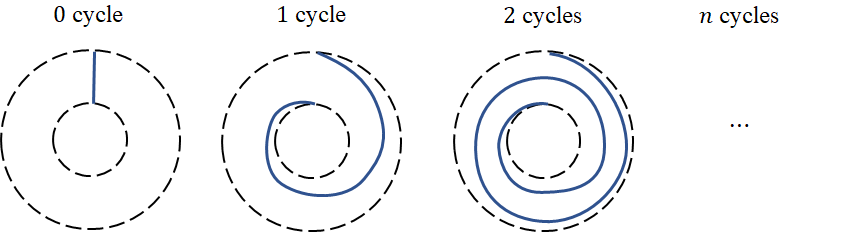
\includegraphics[width = 0.44\textwidth]{figures/proof/fig_cycle}
%\caption{The classification of the cutting paths. One acyclic cutting path corresponds to a family of cyclic cutting paths that share the same start point and end point but go through different cycles.}\label{fig_cycle}
%\end{figure}
%
%\begin{figure}[t]
%\centering
%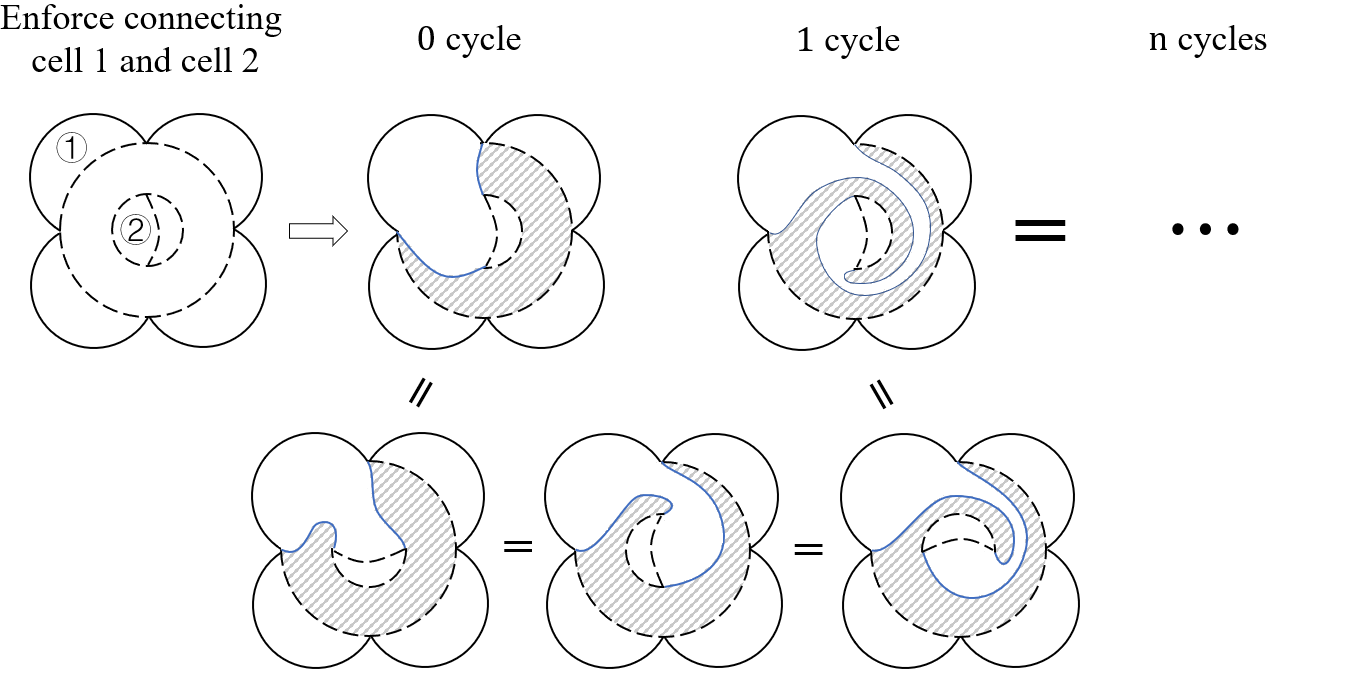
\includegraphics[width = 0.48\textwidth]{figures/proof/fig_no_cyclic_cutting_path}
%\caption{The cyclic cutting paths can be safely disregarded because they serve as the same function as the acyclic cutting paths in the sense of topological structure. The grey cell is the created sub-cell (here only one sub-cell is created). 
%The below three figures show a continuous transformation (rotation) from the $1$-cycle division and $0$-cycle division. The result is easy to generalize to $n$-cycles cases. }\label{fig_no_cyclic_cutting_path}
%\end{figure}
\begin{figure}[t]
\centering
\subfigure[Each acyclic cutting path corresponds to a family of cyclic cutting paths that go through different cycles.]{
	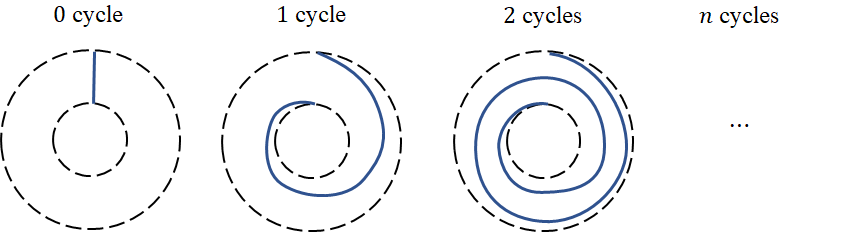
\includegraphics[width = 0.44\textwidth]{figures/proof/fig_cycle}
	\label{fig_cycle}}
\subfigure[Continuous transformation between the $0$-cycle division and $1$-cycle division, with similar results for the $n$-cycles case.]{
	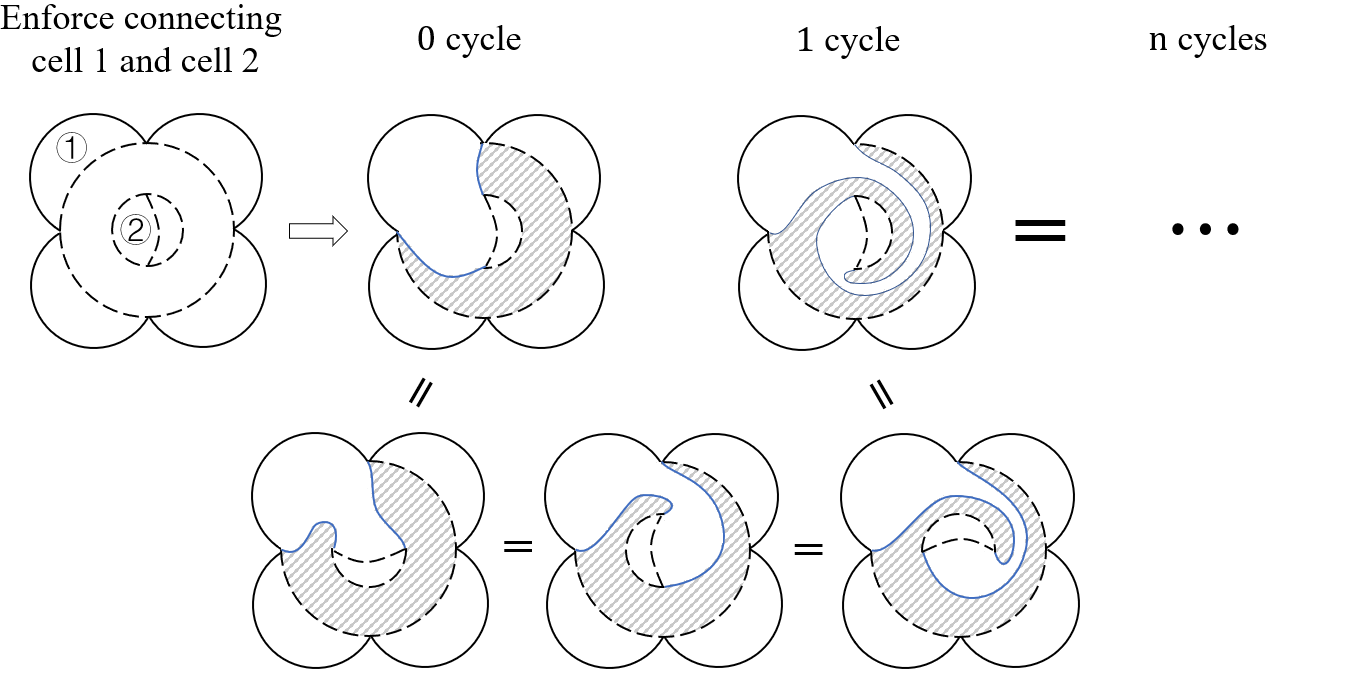
\includegraphics[width = 0.44\textwidth]{figures/proof/fig_no_cyclic_cutting_path}
	\label{fig_no_cyclic_cutting_path}}
\caption{Examples of negligible cutting paths.}
\end{figure}


%\begin{figure}[t]
%\centering
%\subfigure[]{
%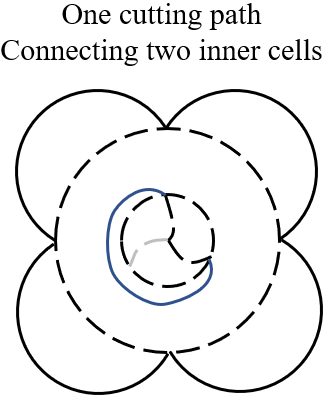
\includegraphics[width=0.14\textwidth]{figures/proof/fig_one_cutting_path_1}
%}
%\subfigure[]{
%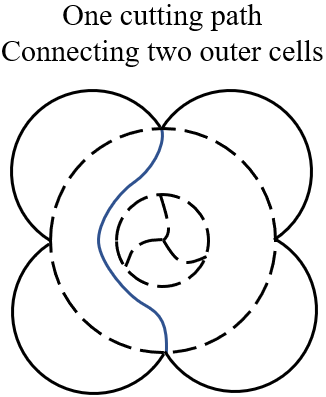
\includegraphics[width=0.14\textwidth]{figures/proof/fig_one_cutting_path_2}
%}
%\subfigure[]{
%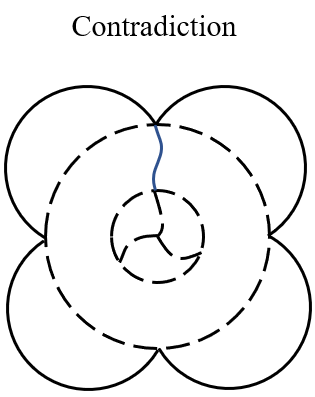
\includegraphics[width=0.14\textwidth]{figures/proof/fig_one_cutting_path_3}\label{fig_one_cutting_path:c}
%}
%\caption{(a) One cutting path can connect two inner cells. (b) One cutting path can connect two outer cells. (c) But one cutting path cannot transform the genus-one cell into simply-connected cells, because the two sides of the cutting path are the same cell, which are impossible to have different colours. }\label{fig_one_cutting_path}
%\end{figure}

%Next, see a counter-example in Fig. \ref{fig_one_cutting_path:c}, where a single cutting path can only lead to contradiction. 
Next, we observe that if there is only one cutting path that connects $\omega$ and $\omega'$, then $\Omega$ is transformed into a 
single simply-connected sub-cell. However, this becomes a contradiction since both sides of the cutting paths are effectively the same cell, 
thus impossible to have different colors. It is therefore apparent that it is not the cutting path but the connected area what determines 
the division of $\Omega$. More precisely, an area connecting the inner part and the outer part of $\Omega$. 
This observation motivates us to directly consider the connectivities between cells. Based on the remarks in 
Section~\ref{section_simply_connected}, we only need to judge whether keeping or removing each edge. 
Let the indices of $J$ edges in $\omega$ and $K$ edges in $\omega'$ be (in cyclic order) 
\begin{equation}\label{equ_omega}
\omega = (\alpha_1, \cdots, \alpha_J)
\end{equation}
\begin{equation}\label{equ_omega_prime}
\omega' = (\alpha'_1, \cdots, \alpha'_K).
\end{equation}
Arbitrarily choosing some edges in $\omega$ and $\omega'$ to generate a connectivity, like
\begin{equation}\label{equ_example_division}
(\{\alpha_{i_1}, \cdots, \alpha_{i_r}\}, \{\alpha'_{j_1}, \cdots, \alpha'_{j_s}\} ), 1\leq r\leq J, 1\leq s\leq K
\end{equation}
where $\{\}$ means the order has no meaning, leads to valid divisions of the $\Omega$. An example is shown in 
Fig.~\ref{fig_not_same_cutting_path}, where it is apparent that results are not unique. The finiteness of this approach is discussed next. 


\subsection{Assignment of Cutting Paths Based on Connectivity}
\label{subsection_arbitrary_assignment}
Extracting all combinations from (\ref{equ_example_division}) does not necessarily mean listing all different divisions. 
In Fig. \ref{fig_not_same_cutting_path}, various divisions are created from the same connectivity. 
%Unlike the simply-connected case, the specified connectivity of a genus-one cell does not determine a unique structure of the cutting paths. For example, in Fig. \ref{fig_not_same_cutting_path}, different divisions are given based on a same connectivity. 
In order to address this issue, the whole division of $\Omega$ is regarded as a two-stage process, first transforming into simply-connected sub-cells and then undertaking further divisions in these sub-cells. 
We prove that in the first stage, only two cutting paths are required which connect $\omega$ and $\omega'$. 

First, all cutting paths that do not connect $\omega$ and $\omega'$ do not appear in the first stage, because they can be seen as further divisions in the generated sub-cells. Refer to Fig.~\ref{fig_equivalence} for an illustration of this phenomenon. 
%Hence, only those cutting paths that connect both $\omega$ and $\omega'$ need further discussion.
Then, let there be three cutting paths that connect $\omega$ and $\omega'$, then $\Omega$ is divided into three simply-connected cells. However, the resulting topological structure is equivalent to $\Omega$ being firstly divided into two sub-cells, then another cutting path creating further divisions iteratively. Hence, there need to be at most two cutting paths in the first-stage.  

In summary, let~$\omega$ and~$\omega'$ be defined by~(\ref{equ_omega}) and~(\ref{equ_omega_prime}), during the first stage a continuous 
subset is identified in~$\omega$, and another one in~$\omega'$. The total number of different divisions is the number of different choices of these continuous subsets. To relieve the problem of the cyclic choices, we enforce the sub-cell $1$ be the one containing $\alpha_1$. 
So all choices in $\omega$ are described by
\begin{equation}\label{equ_all_omega}
\left\{
\begin{aligned}
&\{\alpha_1\}\\
&\{\alpha_1, \alpha_2\}, \{\alpha_J, \alpha_1\}\\
%&\{\alpha_1, \alpha_2, \alpha_3\}, \{\alpha_J, \alpha_1, \alpha_2\}, \{\alpha_{J-1}, \alpha_J, \alpha_1\}\\
&\cdots\\
&\{\alpha_1, \cdots, \alpha_{J-1}\}, \cdots, \{\alpha_3, \cdots, \alpha_J, \alpha_1\}.
\end{aligned}
\right.
\end{equation}
Likewise, all choices in $\omega'$ are given by
\begin{equation}\label{equ_all_omega_prime}
\left\{
\begin{aligned}
&\{\alpha_1'\}, \{\alpha_2'\}, \cdots, \{\alpha_K'\}\\
&\{\alpha_1', \alpha_2'\}, \cdots, \{\alpha_K', \alpha_1'\}\\
%&\{\alpha_1', \alpha_2', \alpha_3'\}, \cdots, \{\alpha_{K}', \alpha_1', \alpha_2'\}\\
&\cdots\\
&\{\alpha_1', \cdots, \alpha_{K-1}'\}, \{\alpha_K', \alpha_1', \cdots, \alpha_{K-2}'\}, \cdots, \{\alpha_2', \cdots, \alpha_K'\}
\end{aligned}
\right.
\end{equation}
%So all choices in $\omega$ and $\omega'$ are
%\begin{align}
%&\left\{
%\begin{aligned}\label{equ_all_omega}
%&\{\alpha_1\}\\
%&\{\alpha_1, \alpha_2\}, \{\alpha_J, \alpha_1\}\\
%&\{\alpha_1, \alpha_2, \alpha_3\}, \{\alpha_J, \alpha_1, \alpha_2\}, \{\alpha_{J-1}, \alpha_J, \alpha_1\}\\
%&\cdots\\
%&\{\alpha_1, \cdots, \alpha_{J-1}\}, \cdots, \{\alpha_3, \cdots, \alpha_J, \alpha_1\}
%\end{aligned}
%\right.\\
%%\end{equation}
%%and all choices in $\omega'$ are
%%\begin{equation}
%&\left\{
%\begin{aligned}\label{equ_all_omega_prime}
%&\{\alpha_1'\}, \{\alpha_2'\}, \cdots, \{\alpha_K'\}\\
%&\{\alpha_1', \alpha_2'\}, \cdots, \{\alpha_K', \alpha_1'\}\\
%&\{\alpha_1', \alpha_2', \alpha_3'\}, \cdots, \{\alpha_{K}', \alpha_1', \alpha_2'\}\\
%&\cdots\\
%&\{\alpha_1', \cdots, \alpha_{K-1}'\}, \{\alpha_K', \alpha_1', \cdots, \alpha_{K-2}'\}, \cdots, \{\alpha_2', \cdots, \alpha_K'\}
%\end{aligned}
%\right.
%\end{align}

\begin{figure}[t]
\centering
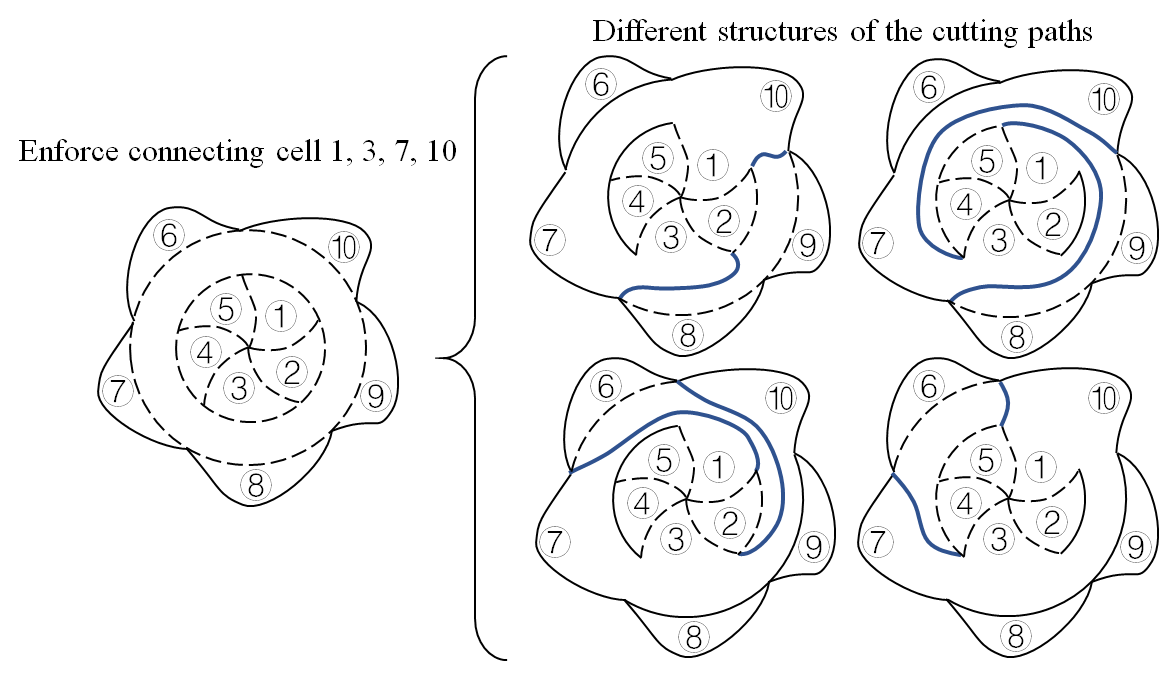
\includegraphics[width = 0.44\textwidth]{figures/proof/fig_only_one_division_3}
\caption{In this example, cells $1$, $3$, $7$ and $10$ are enforced to be connected.
The four distinct divisions shown on the right are all valid, exemplifying the non-uniqueness of the subdivision problem.
%We can see at the right side there are four different divisions having the same function. 
}\label{fig_not_same_cutting_path}
\end{figure}

\begin{figure}[t]
\centering
\subfigure[Illustration of cutting paths that start and end at the same boundary, which can be seen as further divisions (in sub-cell $2$, shown in red).]{
	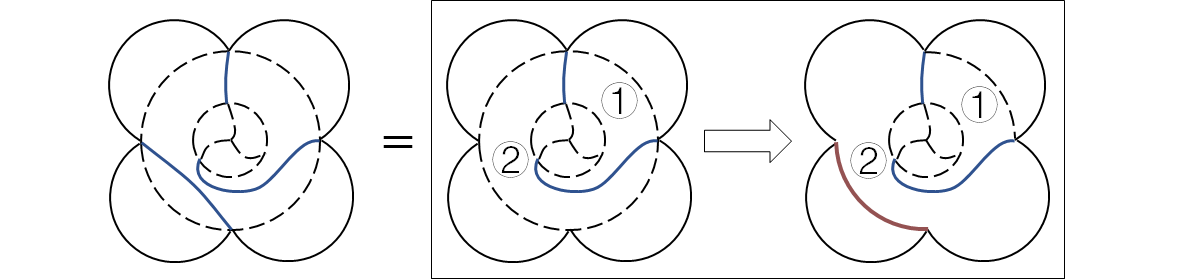
\includegraphics[width=0.43\textwidth]{figures/proof/fig_equivalence_1}}
\subfigure[Example shows that the third (and later) cutting paths connecting $\omega$ and $\omega'$ can be seen as further divisions (in sub-cell $2$, shown in red).]{
	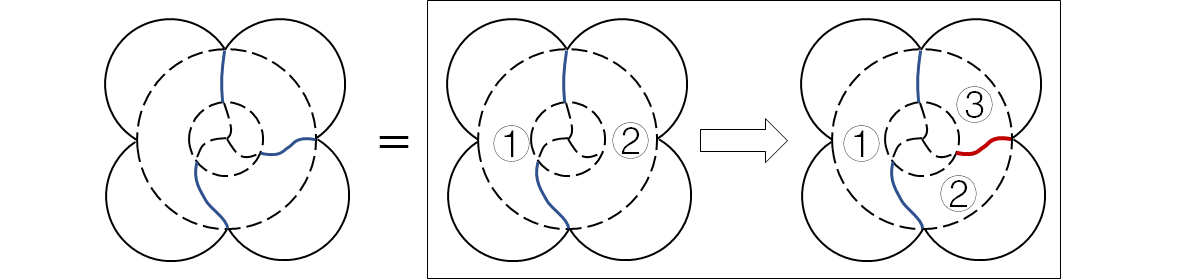
\includegraphics[width=0.43\textwidth]{figures/proof/fig_equivalence_2}}
\caption{The placement of cutting paths can be seen as a two-stage processes: First we only place two cutting paths that connect the inner boundary and the outer boundary, and then place all other cutting paths within the simply-connected sub-cells, seen as further divisions of the sub-cells.}
\label{fig_equivalence}
\end{figure}

\subsection{Complexity Analysis}\label{subsection_genus_one_complexity}
When $\omega$ and $\omega'$ are connected, there are $r$ methods to choose $r$ continuous edges in $\omega$ containing $\alpha_1$, i.e., 
\begin{equation}
\{\alpha_{J-r+1}, \cdots, \alpha_J, \alpha_1\}, \cdots, \{\alpha_1, \cdots, \alpha_r\}
\end{equation}
and $K$ methods to choose $s$ continuous edges in $\omega'$. Summarising all possible $r$ and $s$ we get
\begin{equation}\label{equ_Psi_1}
\Psi(J, K) = \sum\limits_{r = 1}^{J-1}\sum\limits_{s = 1}^{K-1} rK\Phi(r+s)\Phi(J+K -r-s)
\end{equation}
with $\Phi$ defined by~(\ref{equ_Psi}). Moreover, from Section \ref{subsection_un_inner_cell}, the number of different divisions keeping a genus-one structure is 
\begin{equation}\label{equ_Phi_0}
\Phi_0(J, K) = \Phi(J) + \Phi(K) = 2^J + 2^K
\end{equation}
hence the total number of different divisions for a genus-one cell with $J$ edges in the inner boundary and $K$ edges in the outer boundary is given by
\begin{equation}
\Phi(J, K) = \Phi_0(J, K) + \Psi(J, K)
\end{equation}

\section{Solution of Large Genus Cells}
\label{section_large_genus}
There are $n$ inner boundaries in a genus-$n$ cell. Taking the outer boundary into consideration, there are $C_{n+1}^2$ 
possible ``starting-  ending-point" pairs for the possible cutting paths, which are impractical to enumerate and deal with. 
Hence, a multi-stage iterative strategy is once again proposed to transform a genus-$n$ cell into sub-cells with genus no more than $n-1$. 

\subsection{Genus-Two Cell Case}
Following a deduction process similar to the one in Section~\ref{subsection_un_inner_cell}), the ensuing equivalence states arise:
\begin{enumerate}
\item The disconnected inner part can be safely discarded and the remaining becomes a genus-one cell which has been proved solvable. 
After solving both the genus-one cell and the unconnectable part independently, we can arbitrarily place the resulting division of the 
disconnected inner part in the result of the genus-one cell. 
\item When both inner parts are unconnectable, the genus-two cell can be seen as three simply-connected parts. And the solution comes from the arbitrary placements of the solution of the inner parts in the result of the outer part. 
\end{enumerate}

For a genus-$n$ cell, if any of its inner part is disconnected, the genus-$n$ problem becomes a genus-$(n-1)$ problem which is proven solvable under induction. Hence, in this section the focus is on the case when all boundaries are forced to be connected. 

\begin{comment}
Following a deduction process similar to the one in Section~\ref{subsection_un_inner_cell}), the ensuing equivalence states arise:
\begin{enumerate}
\item The disconnected inner part can be safely discarded and the remaining becomes a genus-one cell which has been proved solvable. 
After solving both the genus-one cell and the unconnectable part independently, their solutions can be directly merged to form all solutions of 
a genus-two cell.
\item When both inner parts are unconnectable, the solution of the genus-two cell comes from the direct merging of the solutions of three independent parts.  
\end{enumerate}

Above result is obviously true for any genus cells. Hence, in this section the focus is on the case when all boundaries are forced to be connected. 
\end{comment}

%We introduce the notations. 
Following the notation of a genus-one cell, a genus-two cell is denoted by $\Omega$, with its outer boundary described by 
\begin{equation}
\label{equ_omega_genus_two}
\omega = (\alpha_1, \cdots, \alpha_K)
\end{equation}
and the inner boundaries given by
\begin{equation}
\label{equ_omega_genus_two_1}
\omega^1 = (\alpha^1_1, \cdots, \alpha^1_{J_1})
\end{equation}
\begin{equation}
\label{equ_omega_genus_two_2}
\omega^2 = (\alpha^2_1, \cdots, \alpha^2_{J_2})
\end{equation}
where $\alpha_*$ are the edges in each boundary listed in cyclic order. 

\begin{figure}[t]
\centering
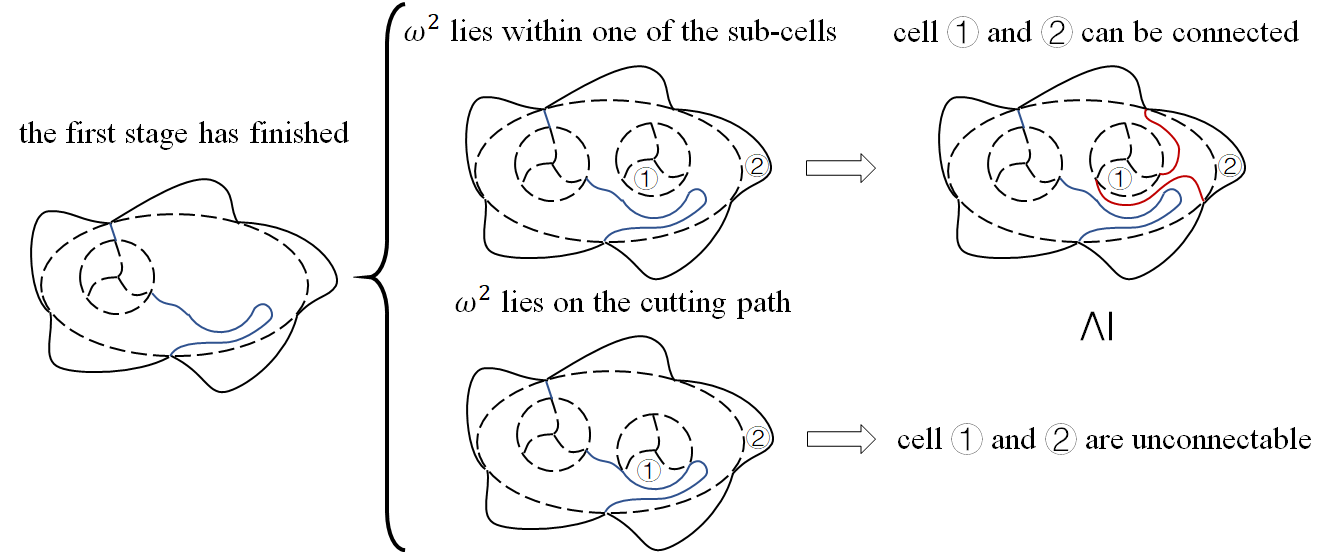
\includegraphics[width = 0.48\textwidth]{figures/proof/fig_no_on_cutting_path}
\caption{Example showing that at each stage, cost-wise it is unnecessary to place the second inner part on the 
cutting paths created earlier (in blue).}
\label{fig_no_on_cutting_path}
\end{figure}

Similar to the process illustrated in 
Section~\ref{section_genus_one}, 
%Fig.~\ref{fig_physical_hole}
%Fig.~\ref{fig_no_on_cutting_path}, 
we regard the whole division of $\Omega$ as a three-stage process. In the first stage, we consider the generation of the cutting paths connecting $\omega$ and $\omega^1$. As per the discussion in 
Section~\ref{subsection_arbitrary_assignment}, at this point there are only two cutting paths, generating two sub-cells. In the second stage, we place $\omega^2$ in each of the sub-cells. In either case, the sub-cell containing $\omega^2$ becomes a genus-one cell. Then it can be solved through further division. After creating other two cutting paths, $\Omega$ is transformed into three simply-connected sub-cells. In the third stage, all other cutting paths are created. 

\subsection{Negligibility of Putting Inner Part on the Cutting Paths}
A special case may first appear to arise when placing $\omega^2$ within each sub-cell generated in the first stage intersecting 
the actual cutting path created (seen in blue in Fig.~\ref{fig_no_on_cutting_path}) 
%unnecessary to consider the place intersecting the generated cutting paths created in the first stage. 
Yet this is a case that requires no consideration given the equivalence shown in the same Figure. 
Since $\omega^2$ is not assumed unconnectable, if a cutting path lies on the existing topological edges, it prevents further connections
(such as the one shown in red in Fig.~\ref{fig_no_on_cutting_path}), leading to higher cost. 
Recalling the result from Section~\ref{subsection_arbitrary_assignment}, there are only two cutting paths dividing $\Omega$ into two parts, so there are exactly two different places to put $\omega^2$, i.e., in either sub-cell created in the first stage. 

\subsection{Complexity Analysis of Solving Genus-2 Cells}
\label{subsection_genus_two_complexity}
When $\omega^1$ and $\omega^2$ are both disconnected, similar to~(\ref{equ_Phi_0}), we have
\begin{equation}\label{equ_Phi_00}
\Phi_{00}(J_1, J_2, K) = 2^{J_1} +2^{J_2} + 2^K
\end{equation}
If $\omega$ and $\omega^1$ are connected, but $\omega^2$ is disconnected, 
\begin{equation}\label{equ_Phi_10}
\Phi_{10}(J_1, J_2, K) = \Psi(J_1, K)+\Phi(J_2)
\end{equation}
exchanging the role of $\omega^1$ and $\omega^2$, 
\begin{equation}\label{equ_Phi_01}
\Phi_{01}(J_1, J_2, K) = \Psi(J_2, K) + \Phi(J_1)
\end{equation}

When both $\omega^1$ and $\omega^2$ are connected, the complexity can be calculated by considering $\omega^2$ being placed in 
different sub-cells separately. Using $\Xi_1$ for the situations that $\omega^2$ is placed in sub-cell $1$, 
and $\Xi_2$ for sub-cell $2$ give rise to
%Assume that in the first stage, $r_1$ edges from $\omega^1$ and $s$ edges from $\omega$ are chosed to form sub-cell $1$, then the number of divisions in the second stage is
\begin{equation}
\Xi_{1}(J_2; r_1, J_1, s, K) = \Psi(J_2, r_1+s)\Phi(J_1+K-r_1-s)
\end{equation}
\begin{equation}
\Xi_{0}(J_2; r_1, J_1, s, K) = \Phi(r_1+s)\Psi(J_2, J_1+K-r_1-s)
\end{equation}
%\begin{equation}
%\Phi_1(J_2, r_1+s)2^{J+K-r_1-s} + 2^{r_1+s}\Phi_1(J_2, J+K - r_1 - s)
%\end{equation}
Going through all possible $r_1$ and $s$, we have 
\begin{equation}\label{equ_Phi_11}
\begin{aligned}
\Psi(J_1, &J_2, K) = \sum\limits_{r_1 = 1}^{J_1-1}\sum\limits_{s = 1}^{K-1}\\
&r_1K\left[\Xi_1\left(J_2; r_1, J_1, s, K\right) + \Xi_0\left(J_2; r_1, J_1, s, K\right)\right]
\end{aligned}
\end{equation} 
Summarising (\ref{equ_Phi_00}), (\ref{equ_Phi_10}), (\ref{equ_Phi_01}) and (\ref{equ_Phi_11}), the final result is compouned by
\begin{equation}
\begin{aligned}
\Phi(J_1, J_2, K) =& \Phi_{00}(J_1, J_2, K) + \Phi_{01}(J_1, J_2, K)\\
& + \Phi_{10}(J_1, J_2, K) + \Psi(J_1, J_2, K)
\end{aligned}
\end{equation}

\subsection{Genus-$n$ Cell Case}
Let $\Omega$ be a genus-$n$ cell, with its outer boundary denoted by $\omega$ and inner boundaries denoted by $\omega^1, \cdots, \omega^n$. The edges and their order in each boundary are given by (\ref{equ_omega_genus_two}) and 
\begin{equation}\label{equ_inner_boundaries}
\omega^i = (\alpha^i_1, \cdots, \alpha^i_{J_i}), \forall i = 1, \cdots, n
\end{equation}
Again, we assume that all $\omega^i$ must be connected, or else the disconnected inner parts can be safely discarded, then the genus-$n$ problem becomes a lower-genus problem. 

Similar to our discussion of the genus-two cell, the whole division of a genus-$n$ cell can be seen as an $(n+1)$-stage process. 
At each stage, $\omega^i$ is added to one of the sub-cells, transforming it into a genus-one sub-cell. Then, exactly two new cutting paths are required to transform this sub-cell again into two simply-connected sub-cells. 
%After the $i$-th stage, the original genus-$n$ cell has been divided into $(i+1)$ simply-connected sub-cells, so there are $(i+1)$ possible places to put $\omega^{i+1}$. 
After $n$ stages, $\Omega$ becomes an enssemble of simply-connected sub-cells. The process is illustrated 
by Fig.~\ref{fig_iterative_process}. 

\begin{figure}[t]
\centering
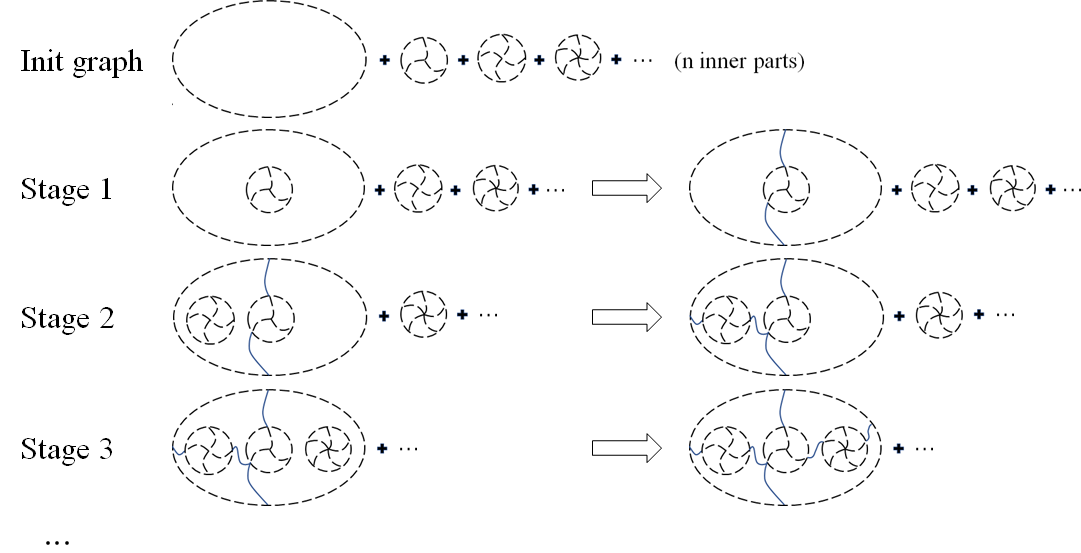
\includegraphics[width=0.48\textwidth]{figures/proof/fig_iterative_process_2}
\caption{Iterative transformation process of the genus-$n$ case.}%This example shows the process of each stage with an assigned connectivity.}
\label{fig_iterative_process}
\end{figure}

%\begin{color}{red}
%(Depends on the page limits) Here we prove that the proposed solution is complete. Given any result division, i.e. sets of cutting paths which transform a genus-$n$ cell into simply-connected sub-cells, we present the corresponding $(n+1)$-stage process to generate it. 
%\end{color}

\subsection{Complexity Analysis of Solving Genus-$n$ Cells}
The number of different divisions can be classified based on whether each inner part is connected. 
For a genus-$n$ cell, define the subscript $T_n$ as a binary string with length $n$, where the digit sum of $T_n$ is $N(T_n)$. 
For example, $N(T_n) = 0$ represents the case that none of the inner boundaries are connected. In this case, 
%If none of the inner boundaries is connected, then $N(T_n)$ = 0
\begin{equation}\label{equ_n_0}
\Phi_{0	\cdots 0}(J_1, \cdots, J_n, K) = 2^{J_1} + \cdots + 2^{J_n} + 2^K
\end{equation} 
If $N(T_n) = 1$, e.g., $\omega$ and $\omega^1$ are connected - and a genus-$(n-1)$ structure is kept after the whole division -  the number of divisions are
%If $\omega^1$ and $\omega$ are connected (thus a genus-$(n-1)$ structure is kept after the whole division process),then ${\rm abs} N$ = 1 the number of different divisions is
\begin{equation}\label{equ_n_1}
\Phi_{1 0 \cdots 0}(J_1, \cdots, J_n, K) = \Psi(J_1, K) + 2^{J_2} + \cdots + 2^{J_n}
\end{equation}
There are $(C_n^1-1)$ terms with $N(T_n)=1$, e.g., $\Phi_{010\cdots 0}$ to $\Phi_{0\cdots 01}$, that can be calculated through exchanging the indices.
Similarily, an example for $N(T_n) = 2$ can be given by 
\begin{equation}\label{equ_n_2}
\Phi_{110\cdots0}(J_1, \cdots, J_n, K) = \Psi(J_1, J_2, K) + 2^{J_3} + \cdots + 2^{J_n}
\end{equation}
and $(C_n^2-1)$ terms can be calculated through exchanging the indices, 
$$\cdots $$
\begin{equation}\label{equ_n_n-1}
\Phi_{1\cdots 10}(J_1, \cdots, J_n, K) = \Psi(J_1, \cdots, J_{n-1}, K) + 2^{J_n}
\end{equation}
with other $(C_n^{n-1}-1)$ similar terms satisfying $N(T_n) = n-1$.

By induction, all the above mentioned terms can be calculated except for the one satisfying $N(T_n) = n$. %with all $1$s in the subscripts. 
After the first stage, we can choose which sub-cell each $\omega^i, i = 2, \cdots, n$ will eventually lie in, and $\Xi_{T_{n-1}}$ are used to consider each situation, with the $i$-th binary digit in $T_{n-1}$ representing that $\omega^i$ lies in sub-cell $1$ or sub-cell $2$. % is $0$ or $1$
Let $B(T, i)$ be the value of the $i$-th digit in $T$,  
\begin{equation}
B(T, i) = \frac{T}{2^{n-i}}\mbox{ mod } 2
\end{equation}
then
\begin{equation}\label{equ_Xi_n}
\begin{aligned}
&\Xi_{T_{n-1}}(J_2, \cdots, J_n; r_1, J, s, K) \\
=&\, \Psi(J_{i_2}, \cdots, J_{i_P}, r_1+s)\Psi(J_{i_{P+1}}, \cdots, J_{i_n}, J+K-r_1-s)
\end{aligned}
\end{equation}
where $i_2, \cdots, i_n$ are specified by
\begin{equation}
\left\{
\begin{aligned}
&B(T_{n-1}, i_j) = 1, &j = 2, \cdots, P\\
&B(T_{n-1}, i_j) = 0, &j = P+1, \cdots, n.
\end{aligned}
\right.
\end{equation}

It is easy to see that the order of $J_{i_*}$ does not effect the result in (\ref{equ_Xi_n}). So
\begin{equation}\label{equ_n_n}
\begin{aligned}
\Psi(J_1, \cdots, &J_n, K) = \sum\limits_{r_1 = 1}^{J_1 - 1} \sum\limits_{s = 1}^{K-1}\\
&\left(r_1K \sum\limits_{T_{n-1} = 0	}^{2^{n-1}-1}\Xi_{T_{n-1}}(J_2, \cdots, J_n; r_1, J, s, K) \right)
\end{aligned}
\end{equation}
Summarising the results from (\ref{equ_n_0}), (\ref{equ_n_1}), (\ref{equ_n_2}), (\ref{equ_n_n-1}), (\ref{equ_n_n}), 
%In summary, let $T$ be a binarial number of length $n$,
\begin{equation}
\begin{aligned}
\Phi(J_1, \cdots, J_n, K) = &\sum\limits_{T_n = 0}^{2^n-2}\Phi_{T_n}(J_1, \cdots, J_n, K)\\
& + \Psi(J_1, \cdots, J_n, K)
\end{aligned}
\end{equation}


\begin{figure}[t]
\centering
\subfigure[]{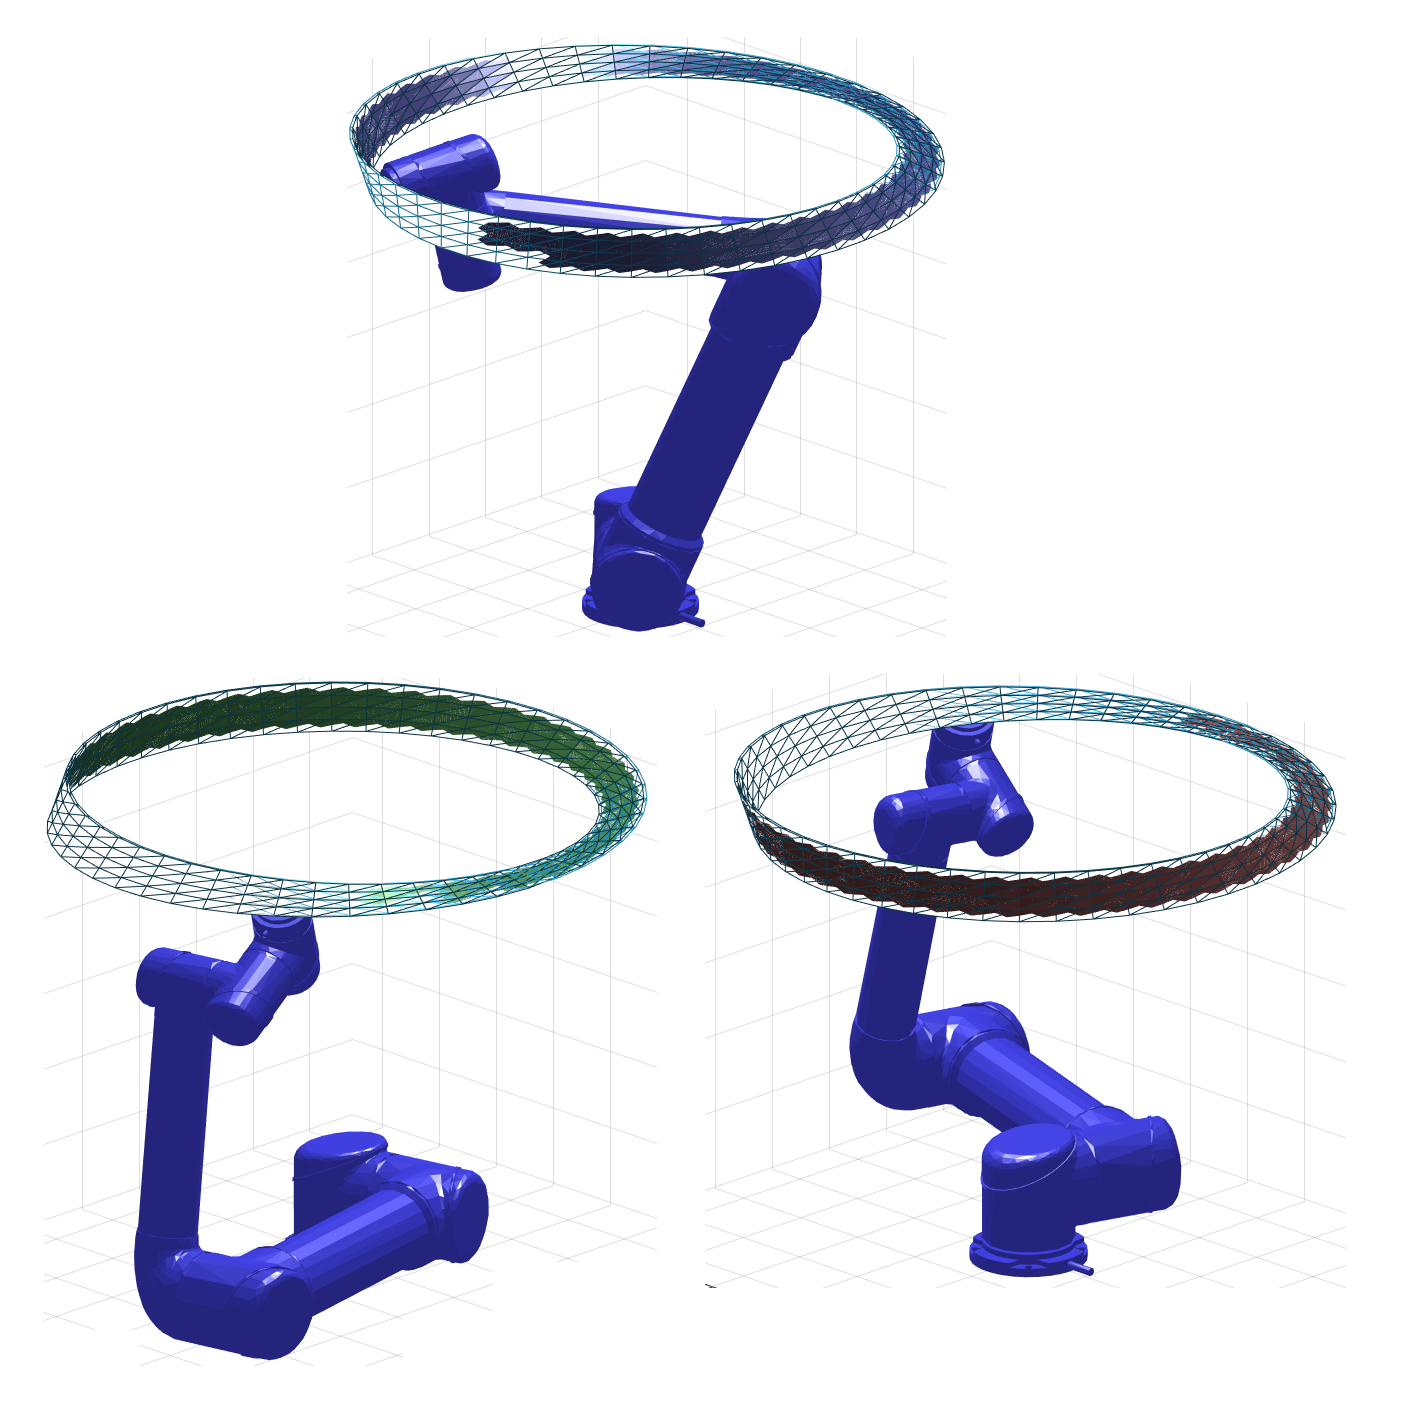
\includegraphics[width = 0.24\columnwidth]{figures/mobius_exp/demo_comb}}
\subfigure[]{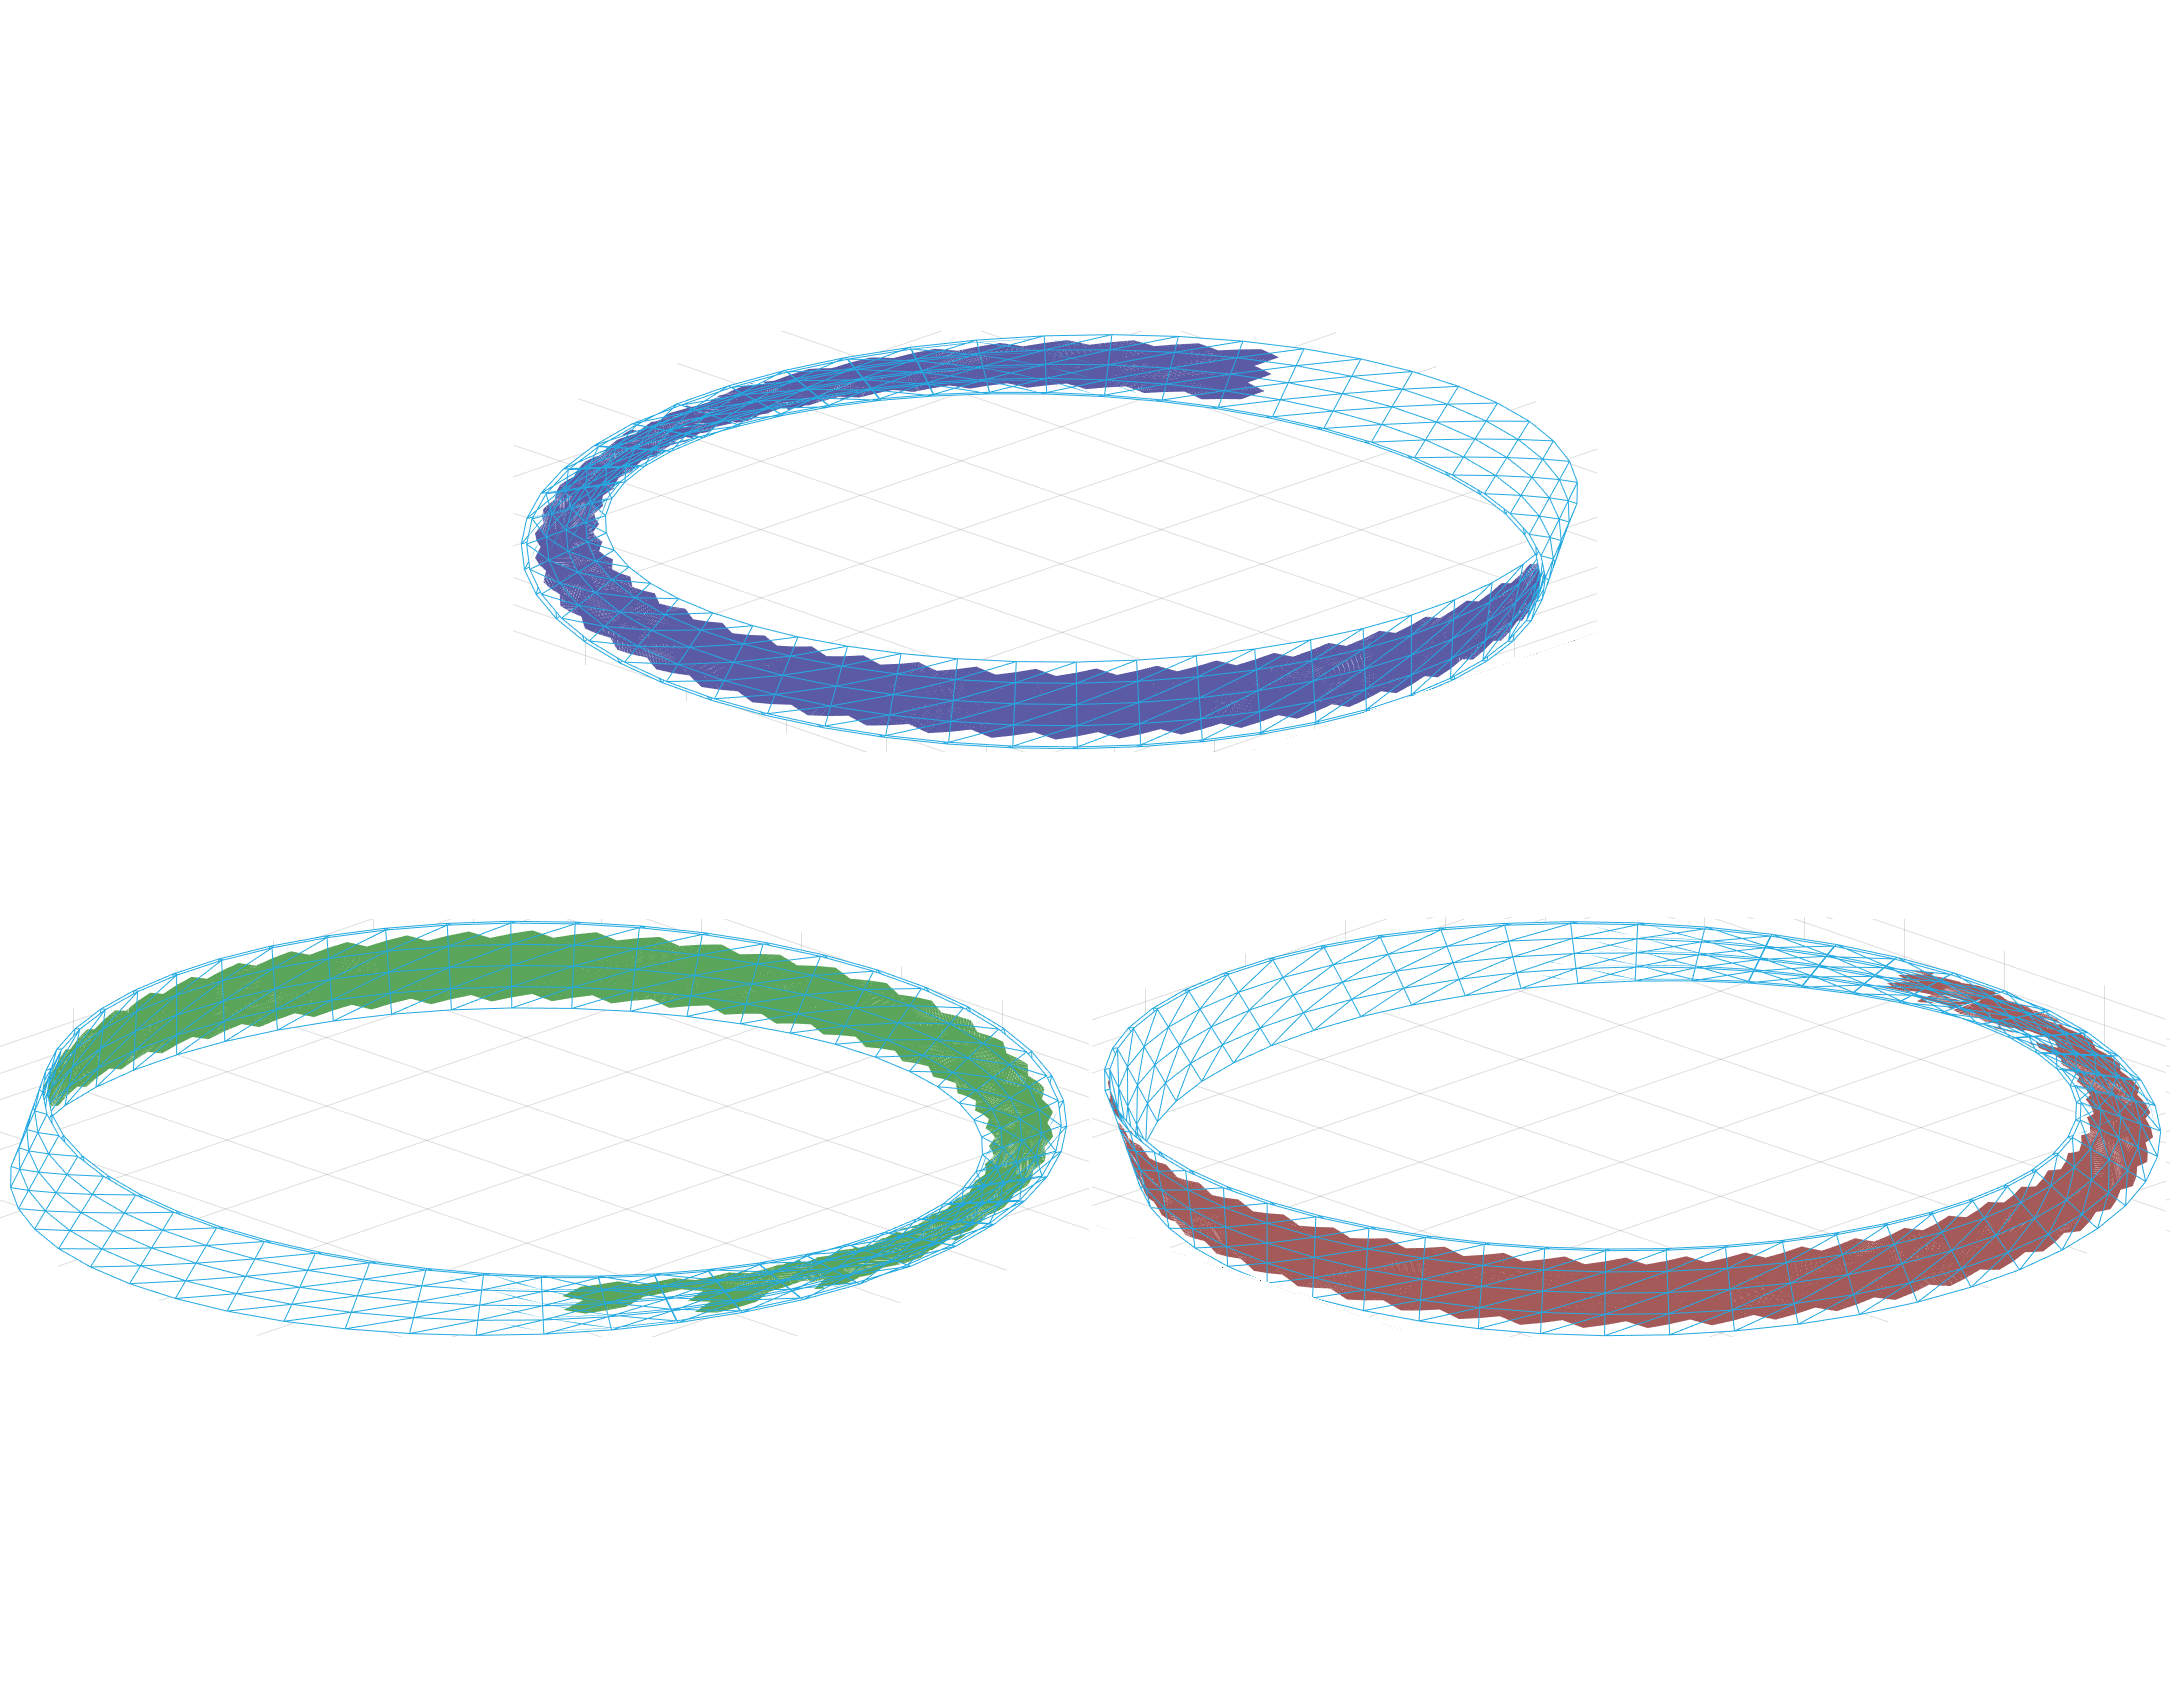
\includegraphics[width = 0.24\columnwidth]{figures/mobius_exp/color_comb}}
\subfigure[]{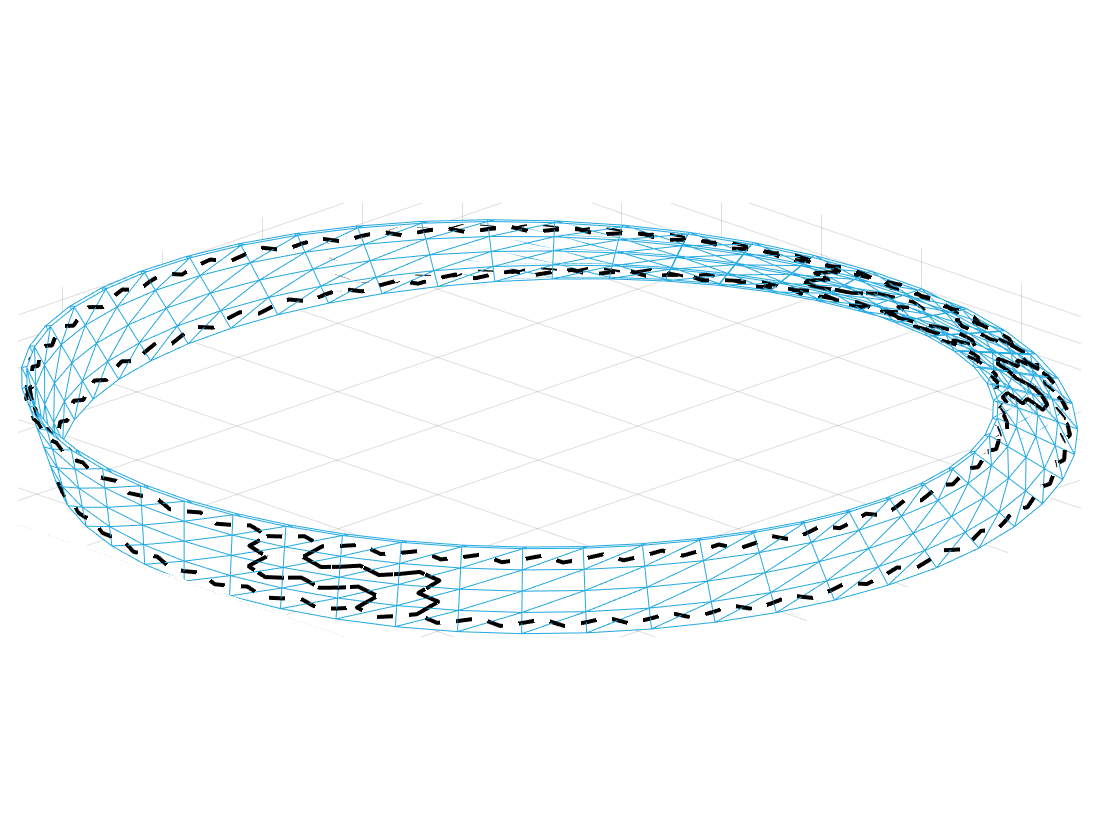
\includegraphics[width = 0.24\columnwidth]{figures/mobius_exp/init_graph}}
\subfigure[]{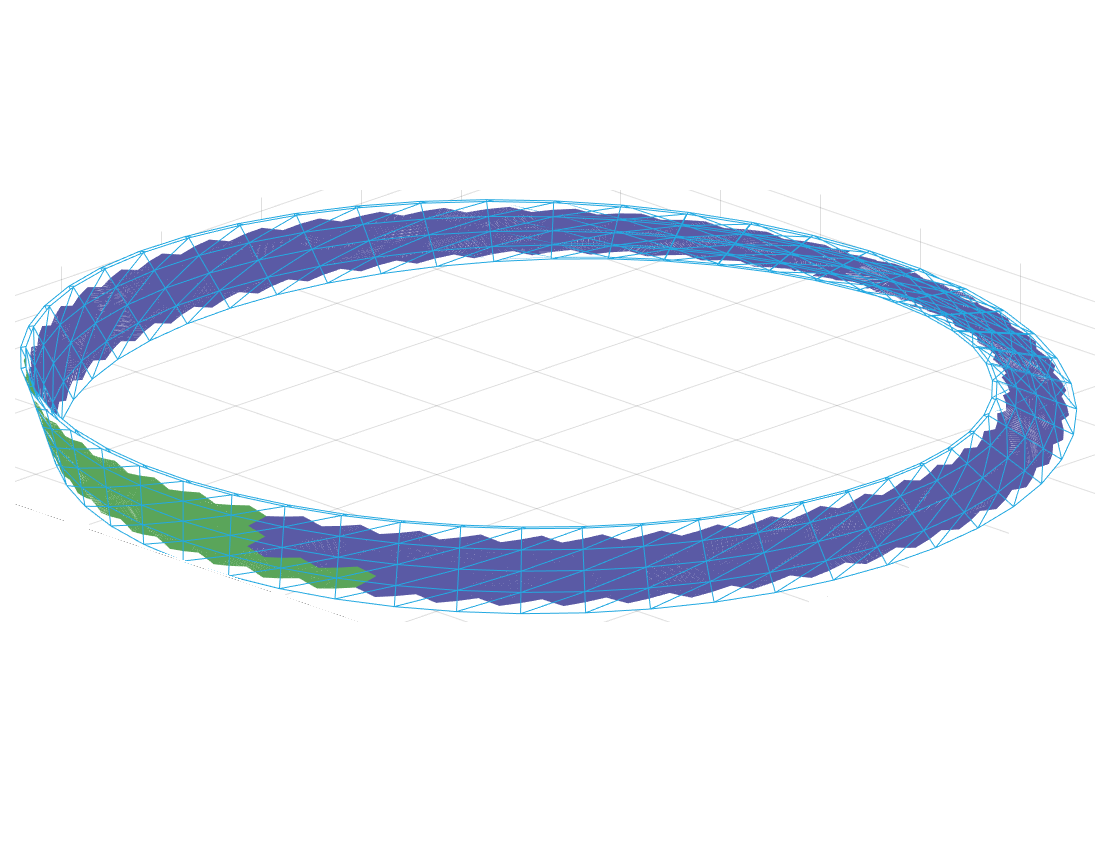
\includegraphics[width = 0.24\columnwidth]{figures/mobius_exp/result_graph}}
\caption{Proposed NCPP applied to a Mobi\"{u}s strip (a) Examples of different configurations. 
(b) Coverable area of each the corresponding (colour) configuration. 
(c) Topological graph (d) One optimal solution requiring $1$ lift-offs. }
\label{fig_mobius_exp}
\end{figure}



\begin{figure}[t]
\centering
\subfigure[]{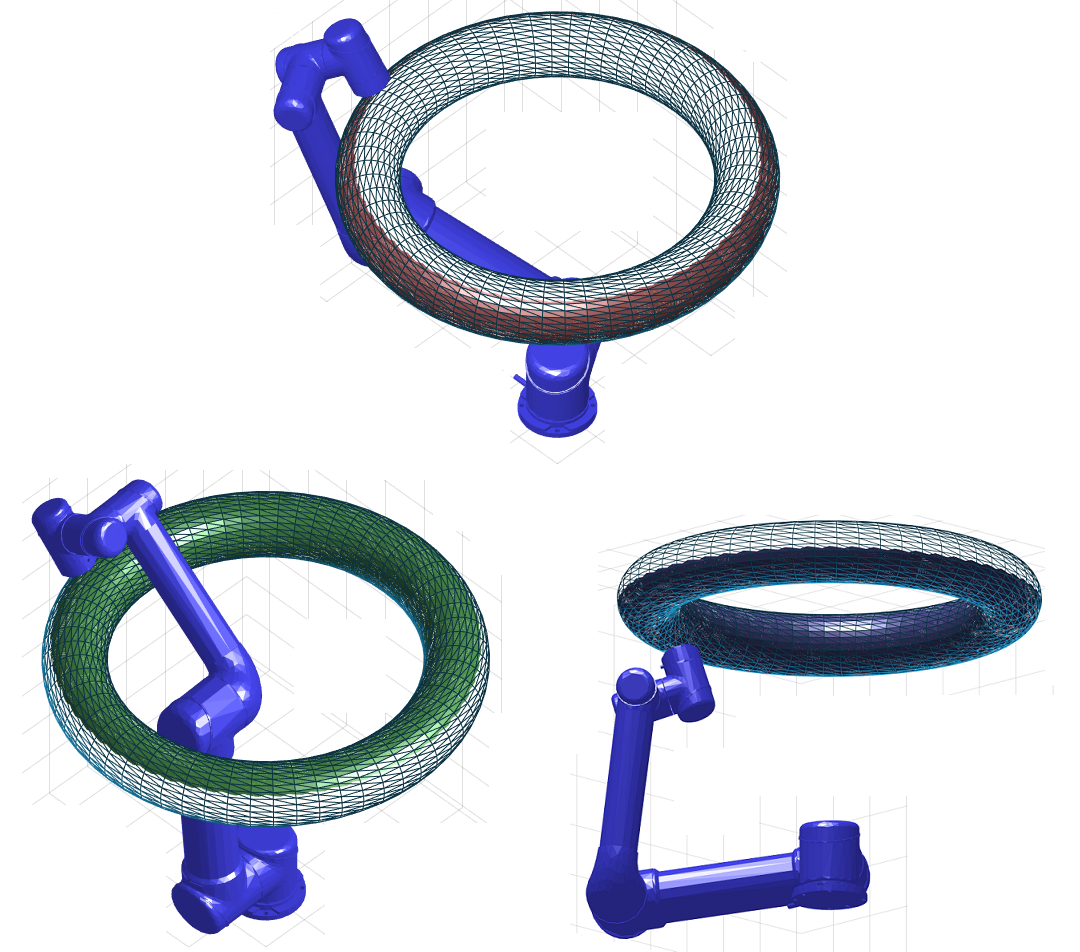
\includegraphics[width = 0.24\columnwidth]{figures/ring_exp/demo_comb}}
\subfigure[]{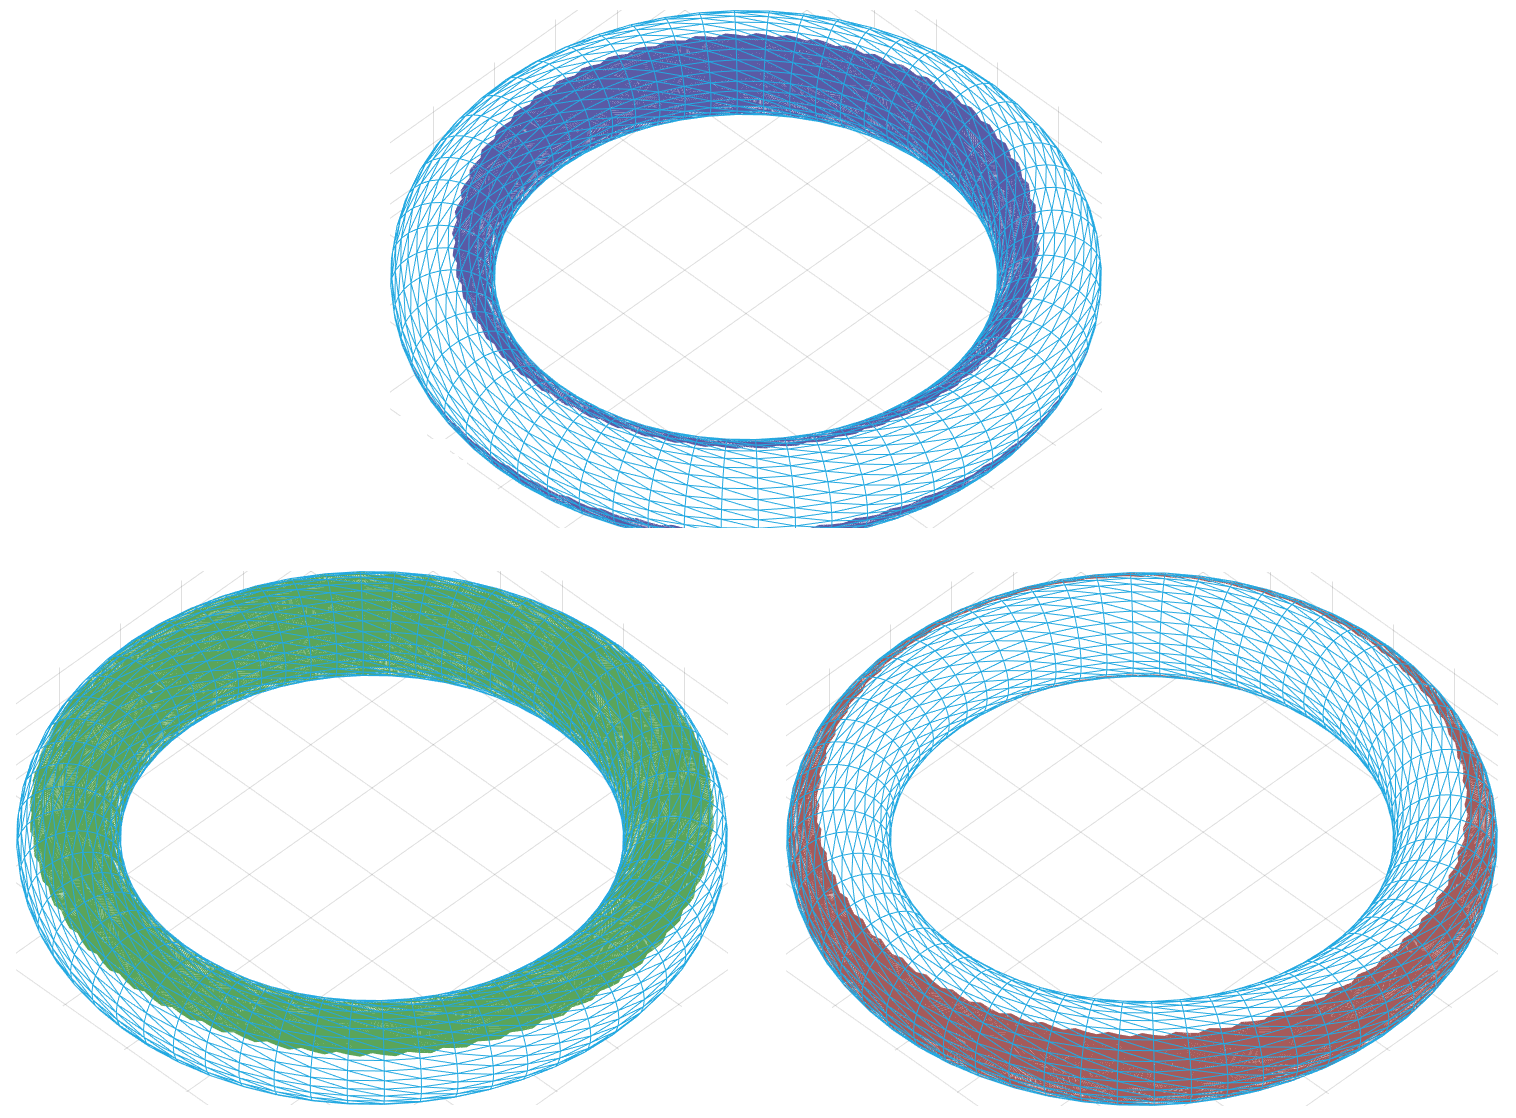
\includegraphics[width = 0.24\columnwidth]{figures/ring_exp/color_comb}}
\subfigure[]{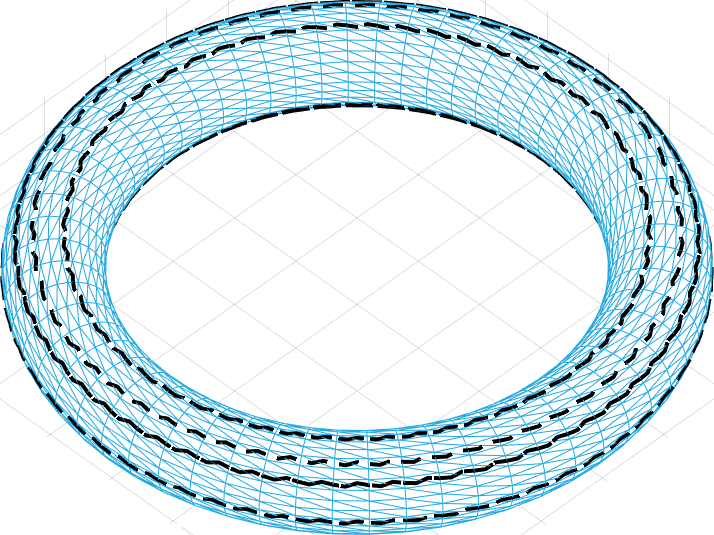
\includegraphics[width = 0.24\columnwidth]{figures/ring_exp/init_graph}}
\subfigure[]{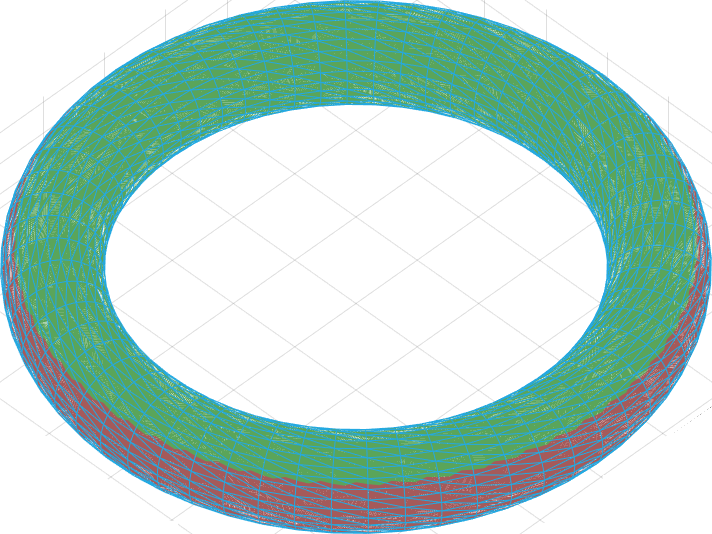
\includegraphics[width = 0.24\columnwidth]{figures/ring_exp/result_graph}}
\caption{Proposed NCPP applied to a closed surface ring(a) Examples of different configurations, where it becomes apparent that significant discontinuities will be inevitable without proper planning should the manipulator motion stretch in and out of the ring.  (b) Continuous coverable area 
of three (colour) configurations, all of them being genus-one cells. (c) Topological graph generated. (d) One optimal solution, where 
only $1$ lift-off is required.}
\label{fig_ring_exp}
\end{figure}



%\begin{figure}[t]
%\centering
%\subfigure[]{
%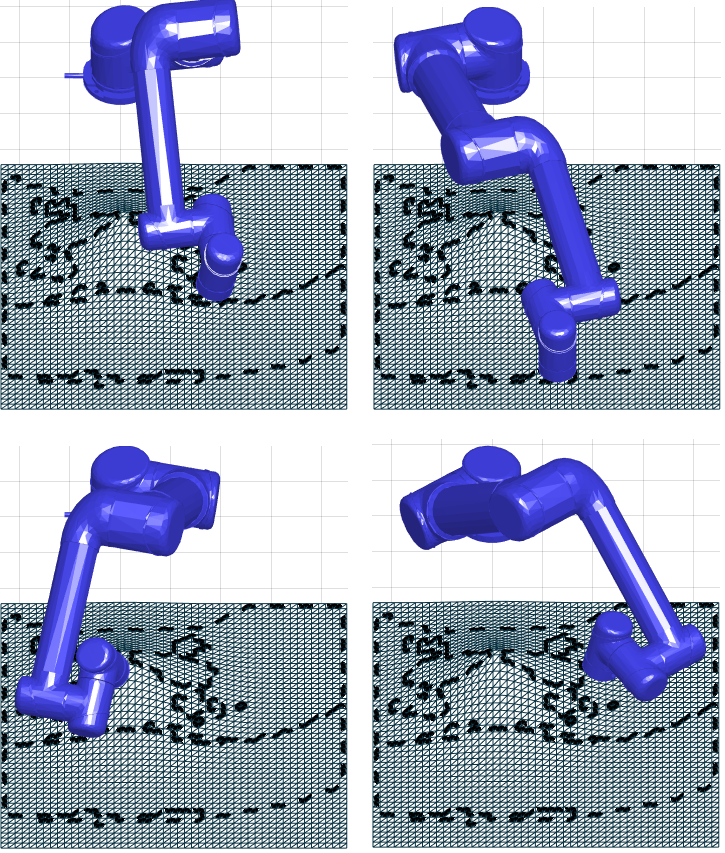
\includegraphics[width = 0.10\textwidth]{figures/hill_exp/0_06/new/hill_demo_comb}
%}
%\subfigure[]{
%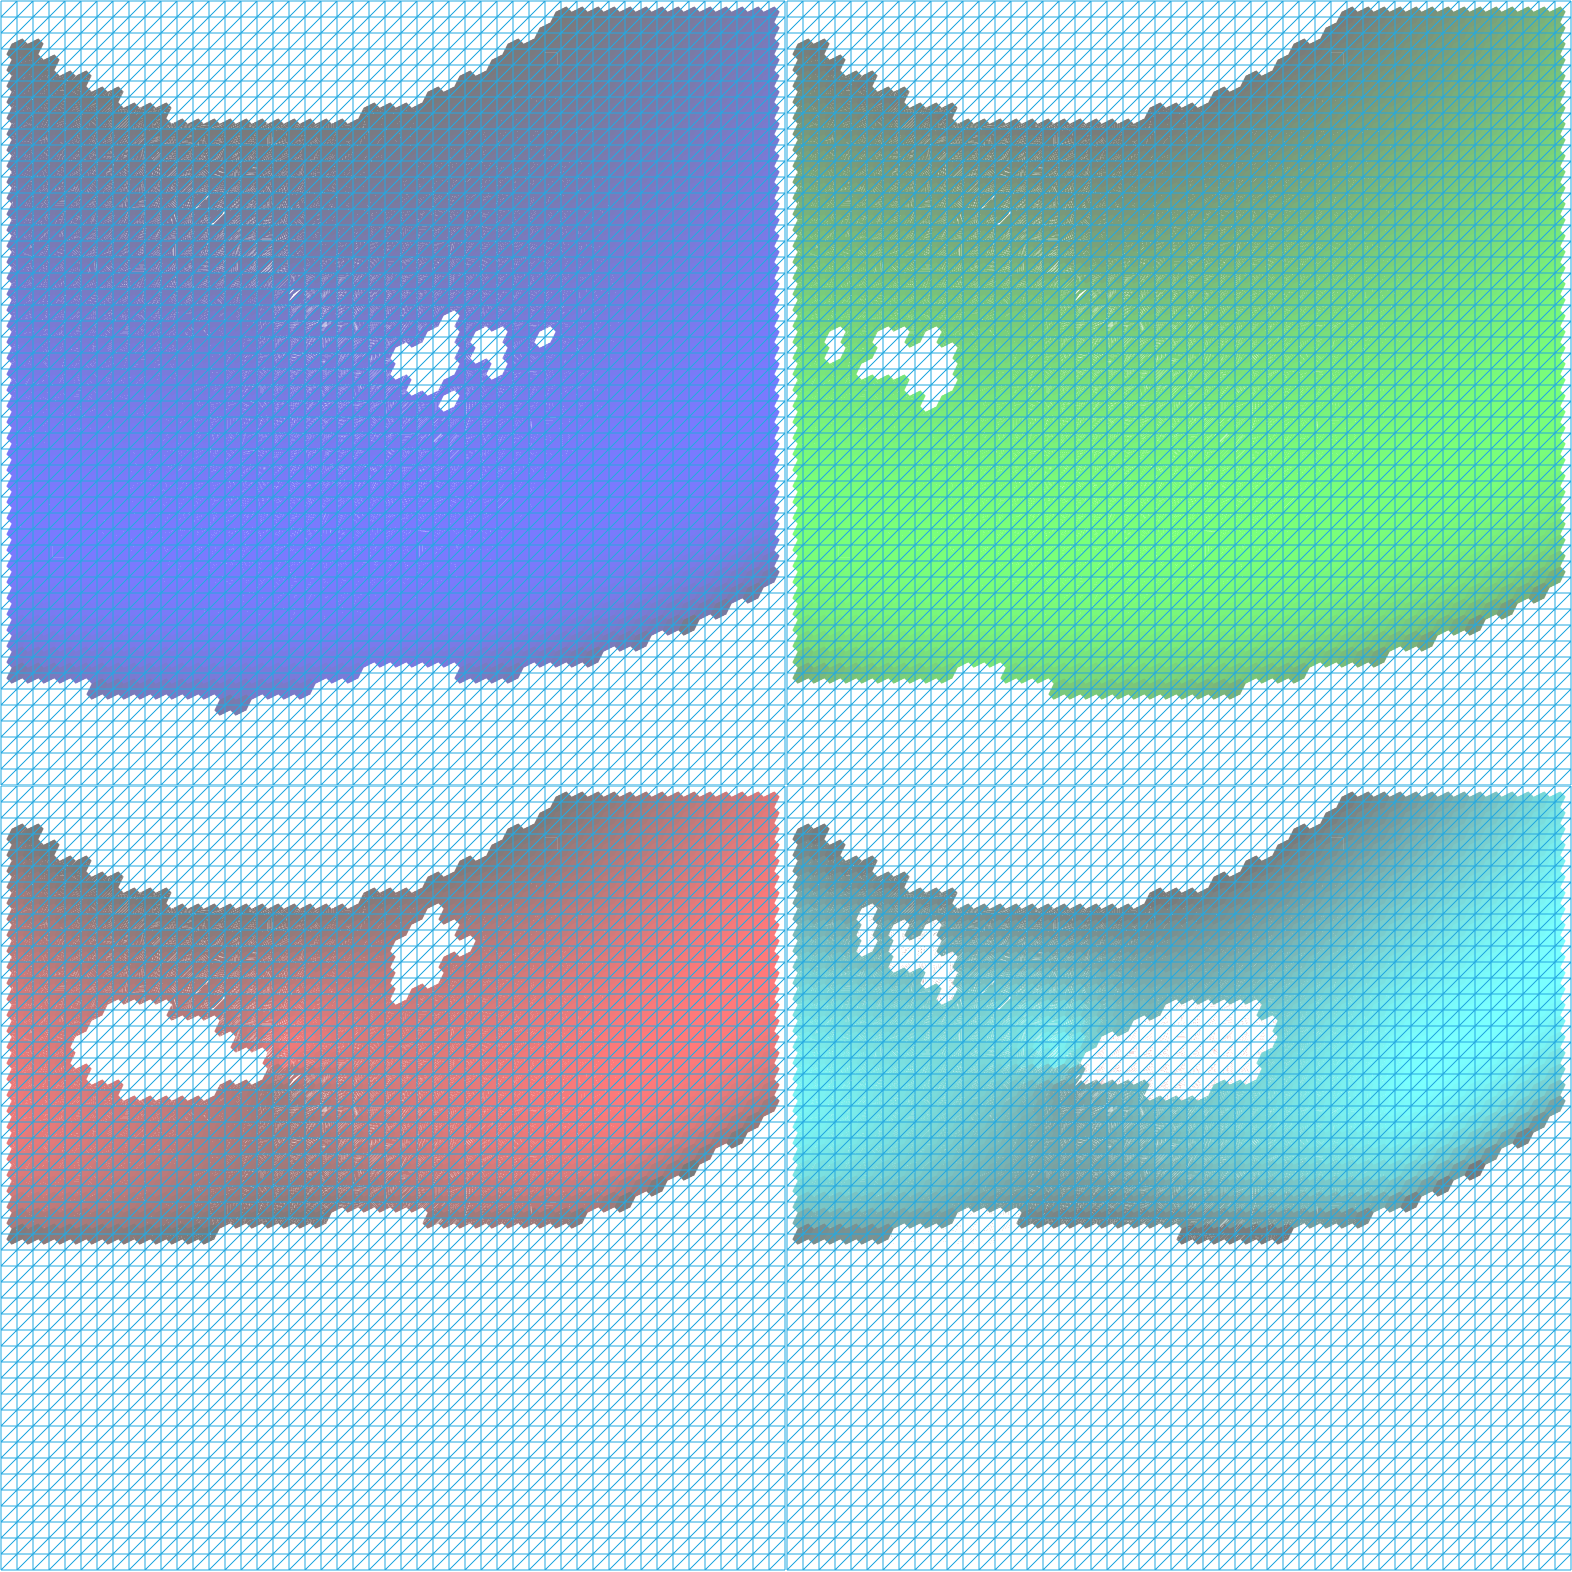
\includegraphics[width = 0.10\textwidth]{figures/hill_exp/0_06/new/color_comb_manipulability}
%}
%\subfigure[]{
%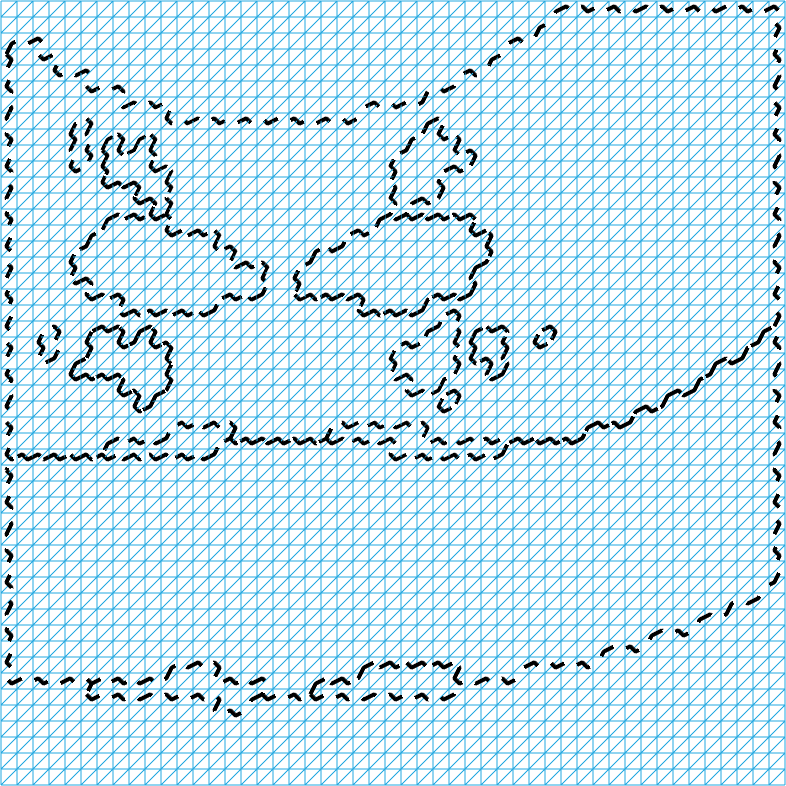
\includegraphics[width = 0.10\textwidth]{figures/hill_exp/0_06/new/init_graph}
%}
%\subfigure[]{
%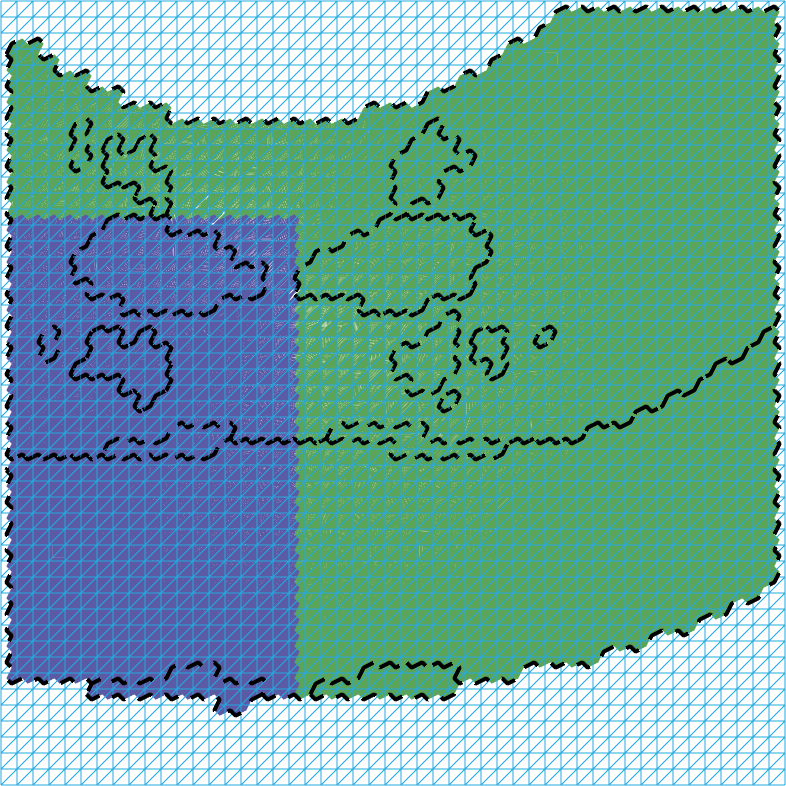
\includegraphics[width = 0.10\textwidth]{figures/hill_exp/0_06/new/result_graph}
%}
%\caption{(a) Examples of different configurations. The configurations shown are near the boundary of their reachable area, because of the collision between the fore-arm and the wrist, or that between the upper-arm and the hill.  (b) Coverable area of the corresponding colours. (c) Topological graph. (d) One optimal solution requiring $1$ lift-offs. }\label{fig_hill_exp_0_06}
%\end{figure}

\begin{figure}[t]
\centering
\subfigure[]{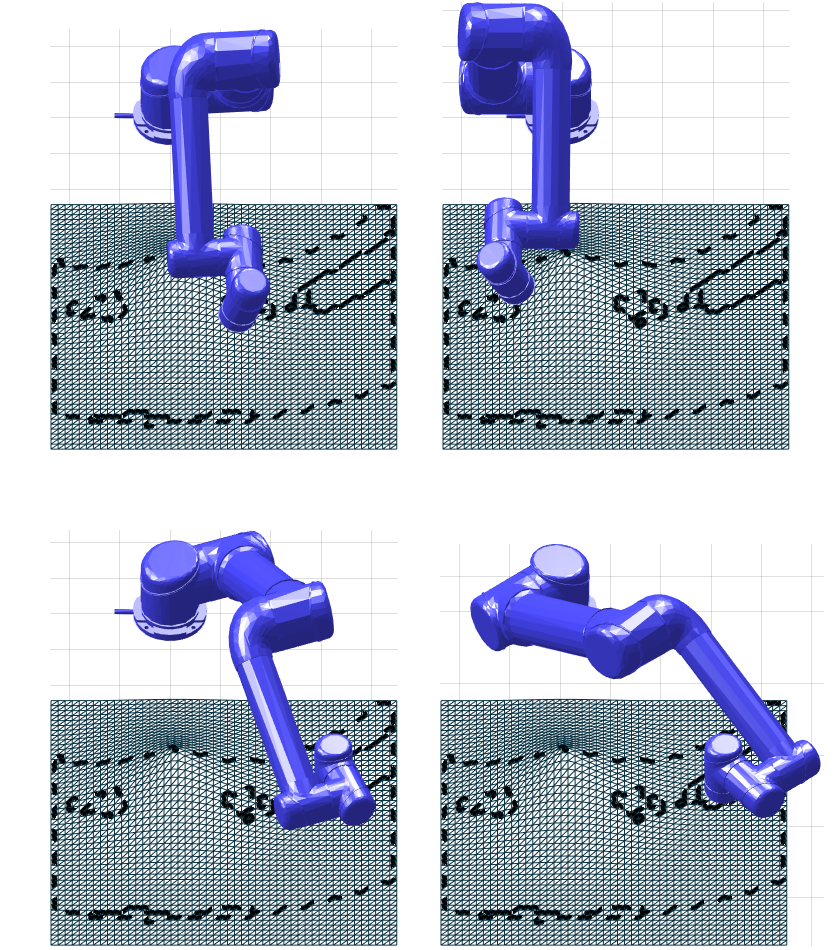
\includegraphics[width = 0.24\columnwidth]{figures/hill_exp/0_10/demo_comb}\label{fig:manip_010_configs}}
\subfigure[]{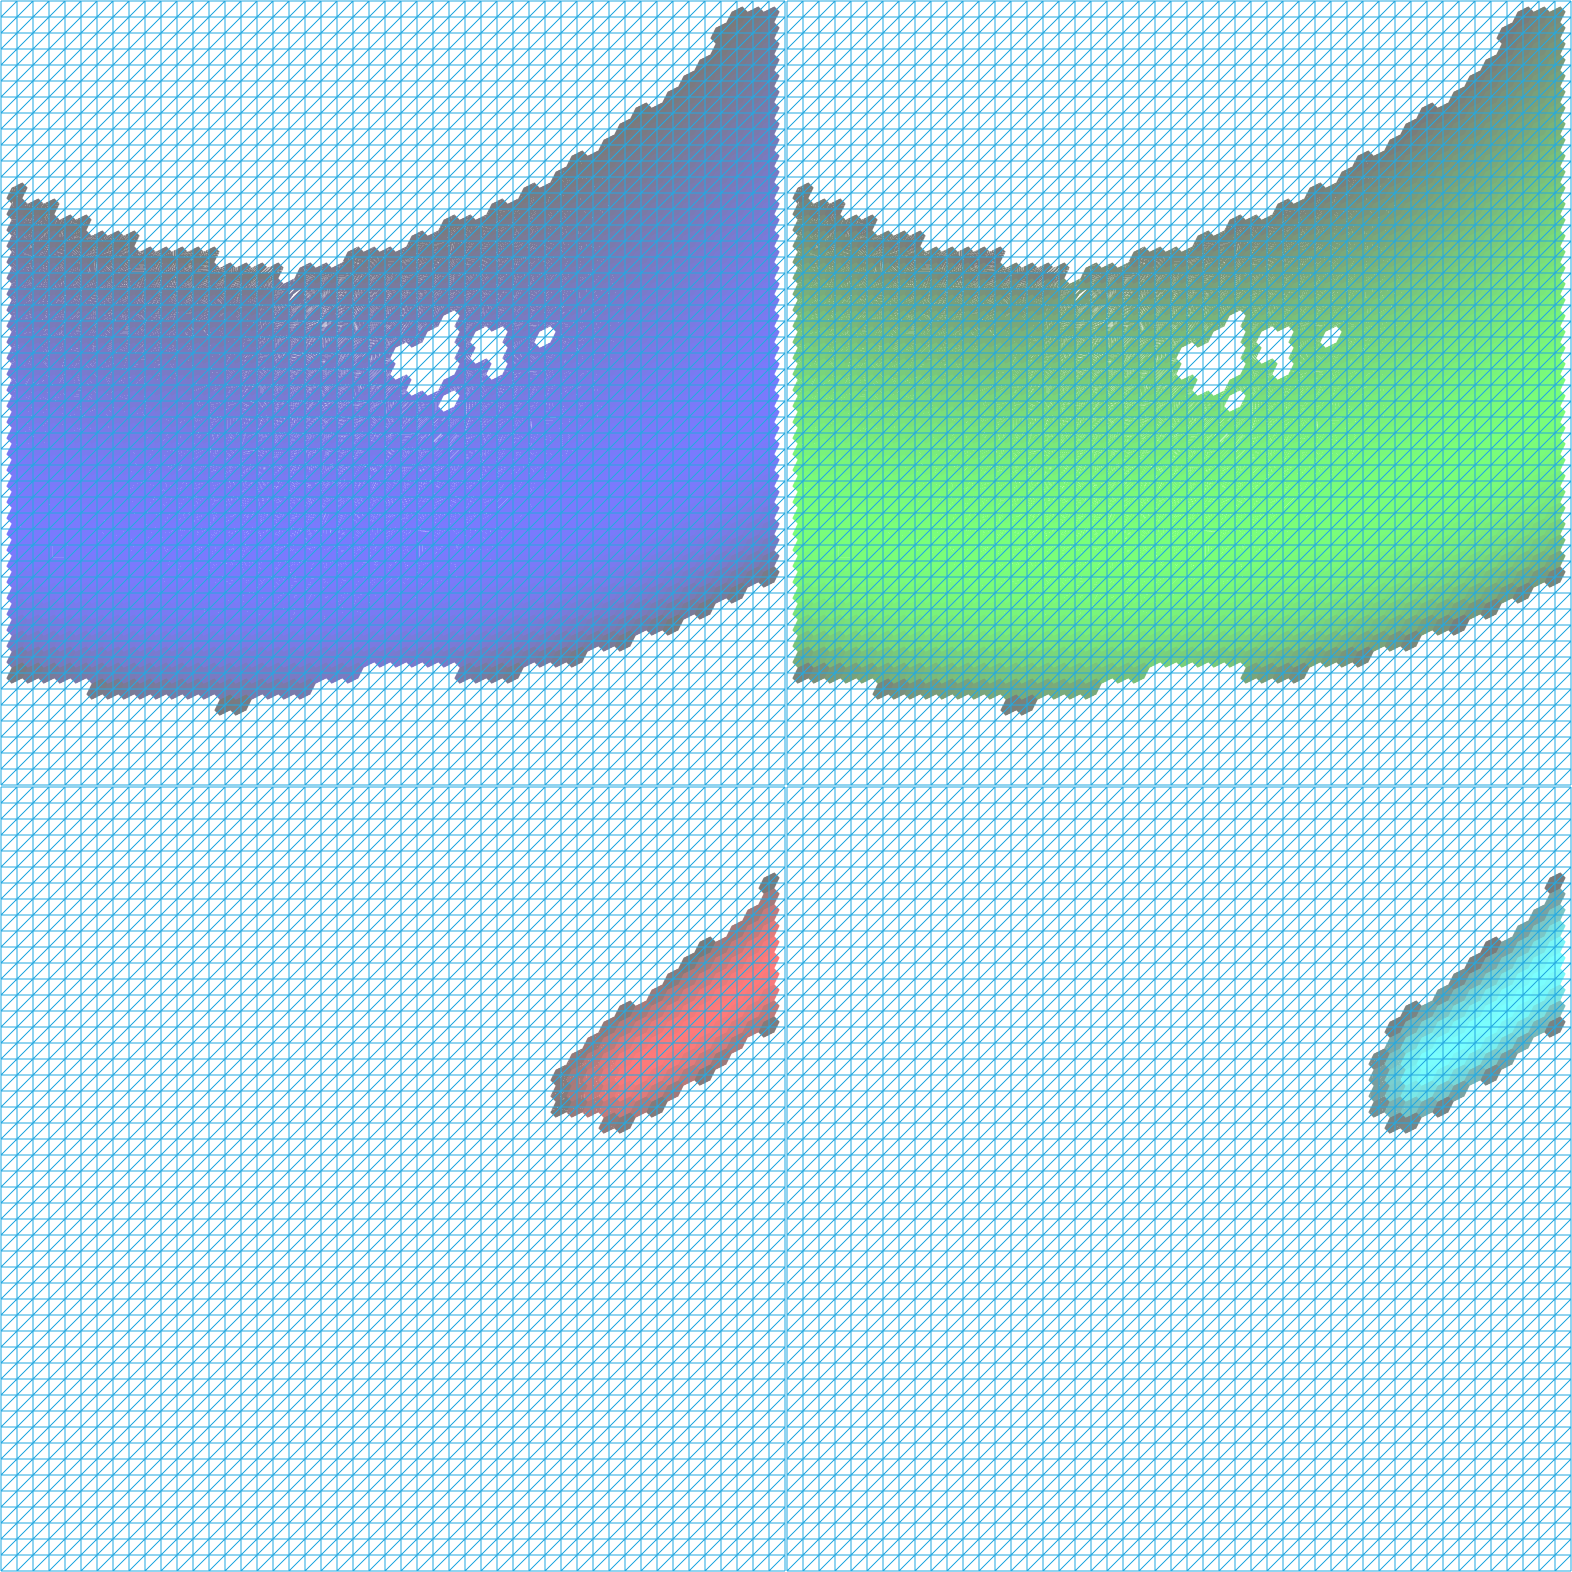
\includegraphics[width = 0.24\columnwidth]{figures/hill_exp/0_10/color_comb_manipulability_with_mesh}}
\subfigure[]{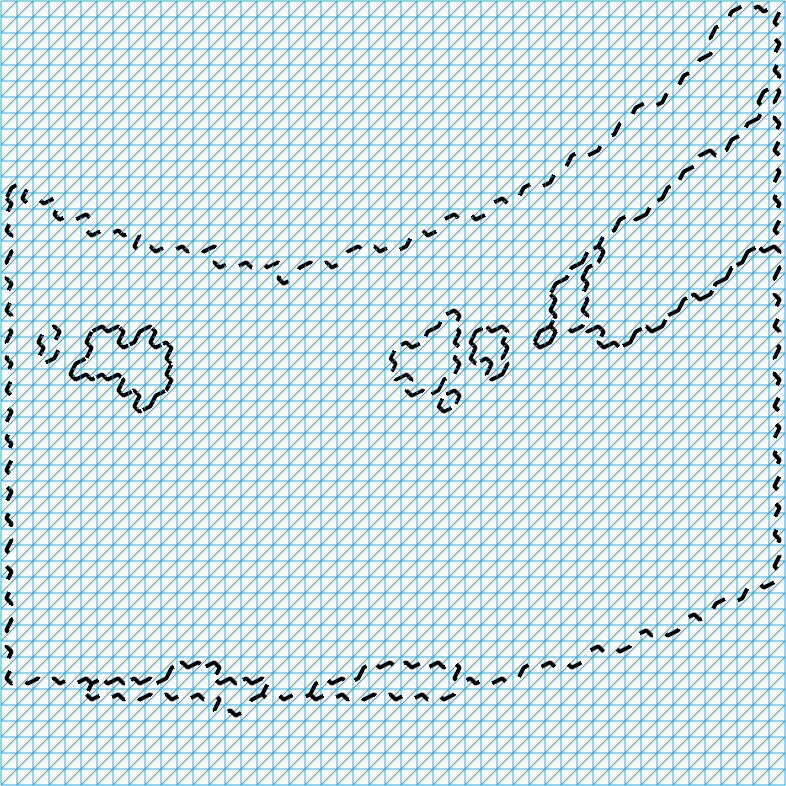
\includegraphics[width = 0.24\columnwidth]{figures/hill_exp/0_10/init_graph}}
\subfigure[]{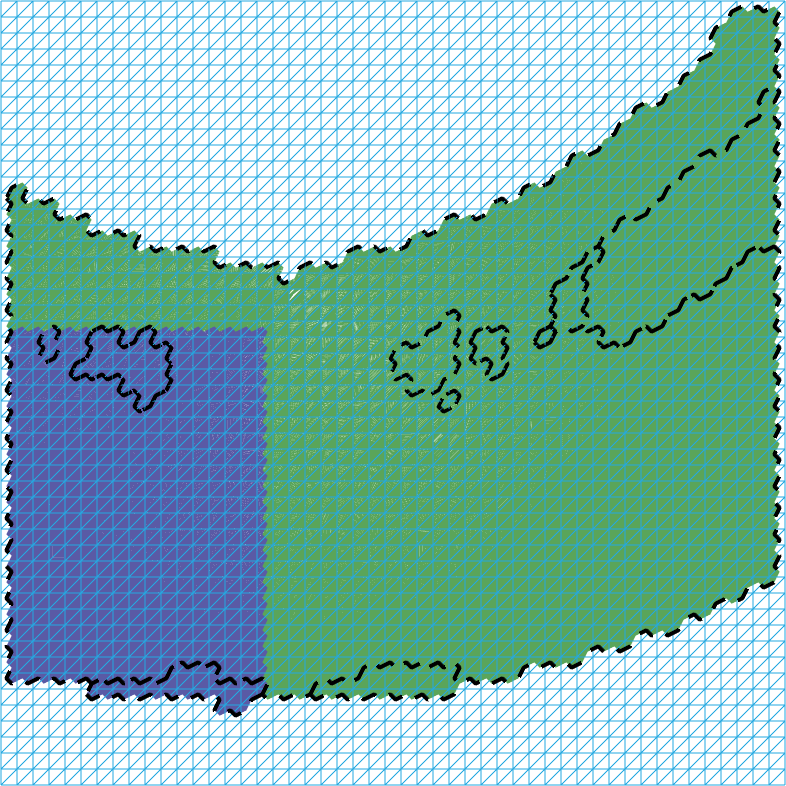
\includegraphics[width = 0.24\columnwidth]{figures/hill_exp/0_10/result_graph}}
\caption{(a) Examples of configurations belonging to different colours, where the threshold of manipulability at each point is set to $>0.1$. 
(b) Coverable area of the corresponding colours. We can see the wrist-flipped configurations can only cover reduced areas, and the configurations 
can no longer reach the area near the base of the manipulator (as compared with Fig.~\ref{fig:hill_multiply_conn}, where the minimum threshold is set to $> 0.06$). (c) Topological graph. (d) An optimal solution with $1$ lift-off. }
\label{fig_hill_exp_0_10}
\end{figure}

\begin{figure}[t]
\centering
\subfigure[]{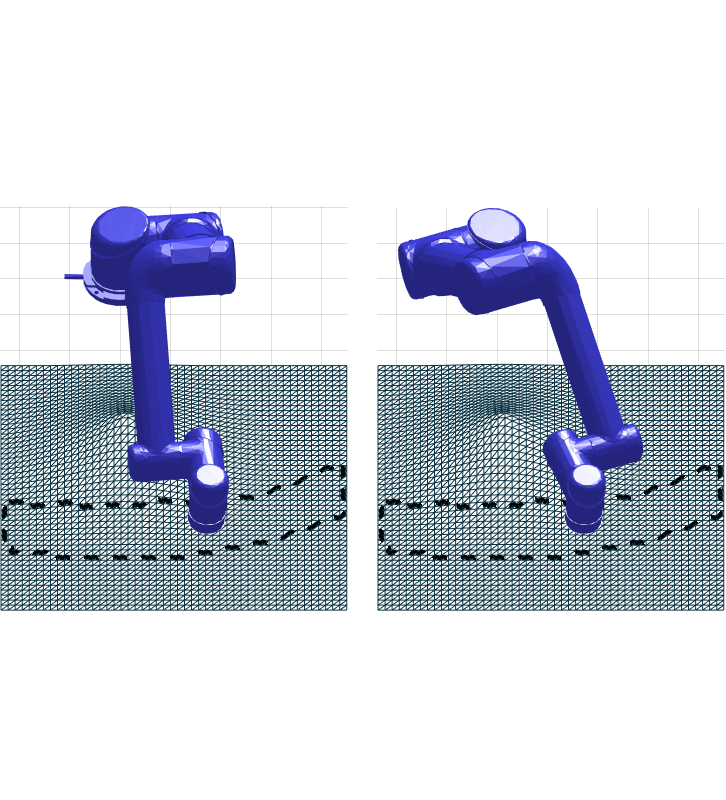
\includegraphics[width = 0.24\columnwidth]{figures/hill_exp/0_16/demo_comb}}
\subfigure[]{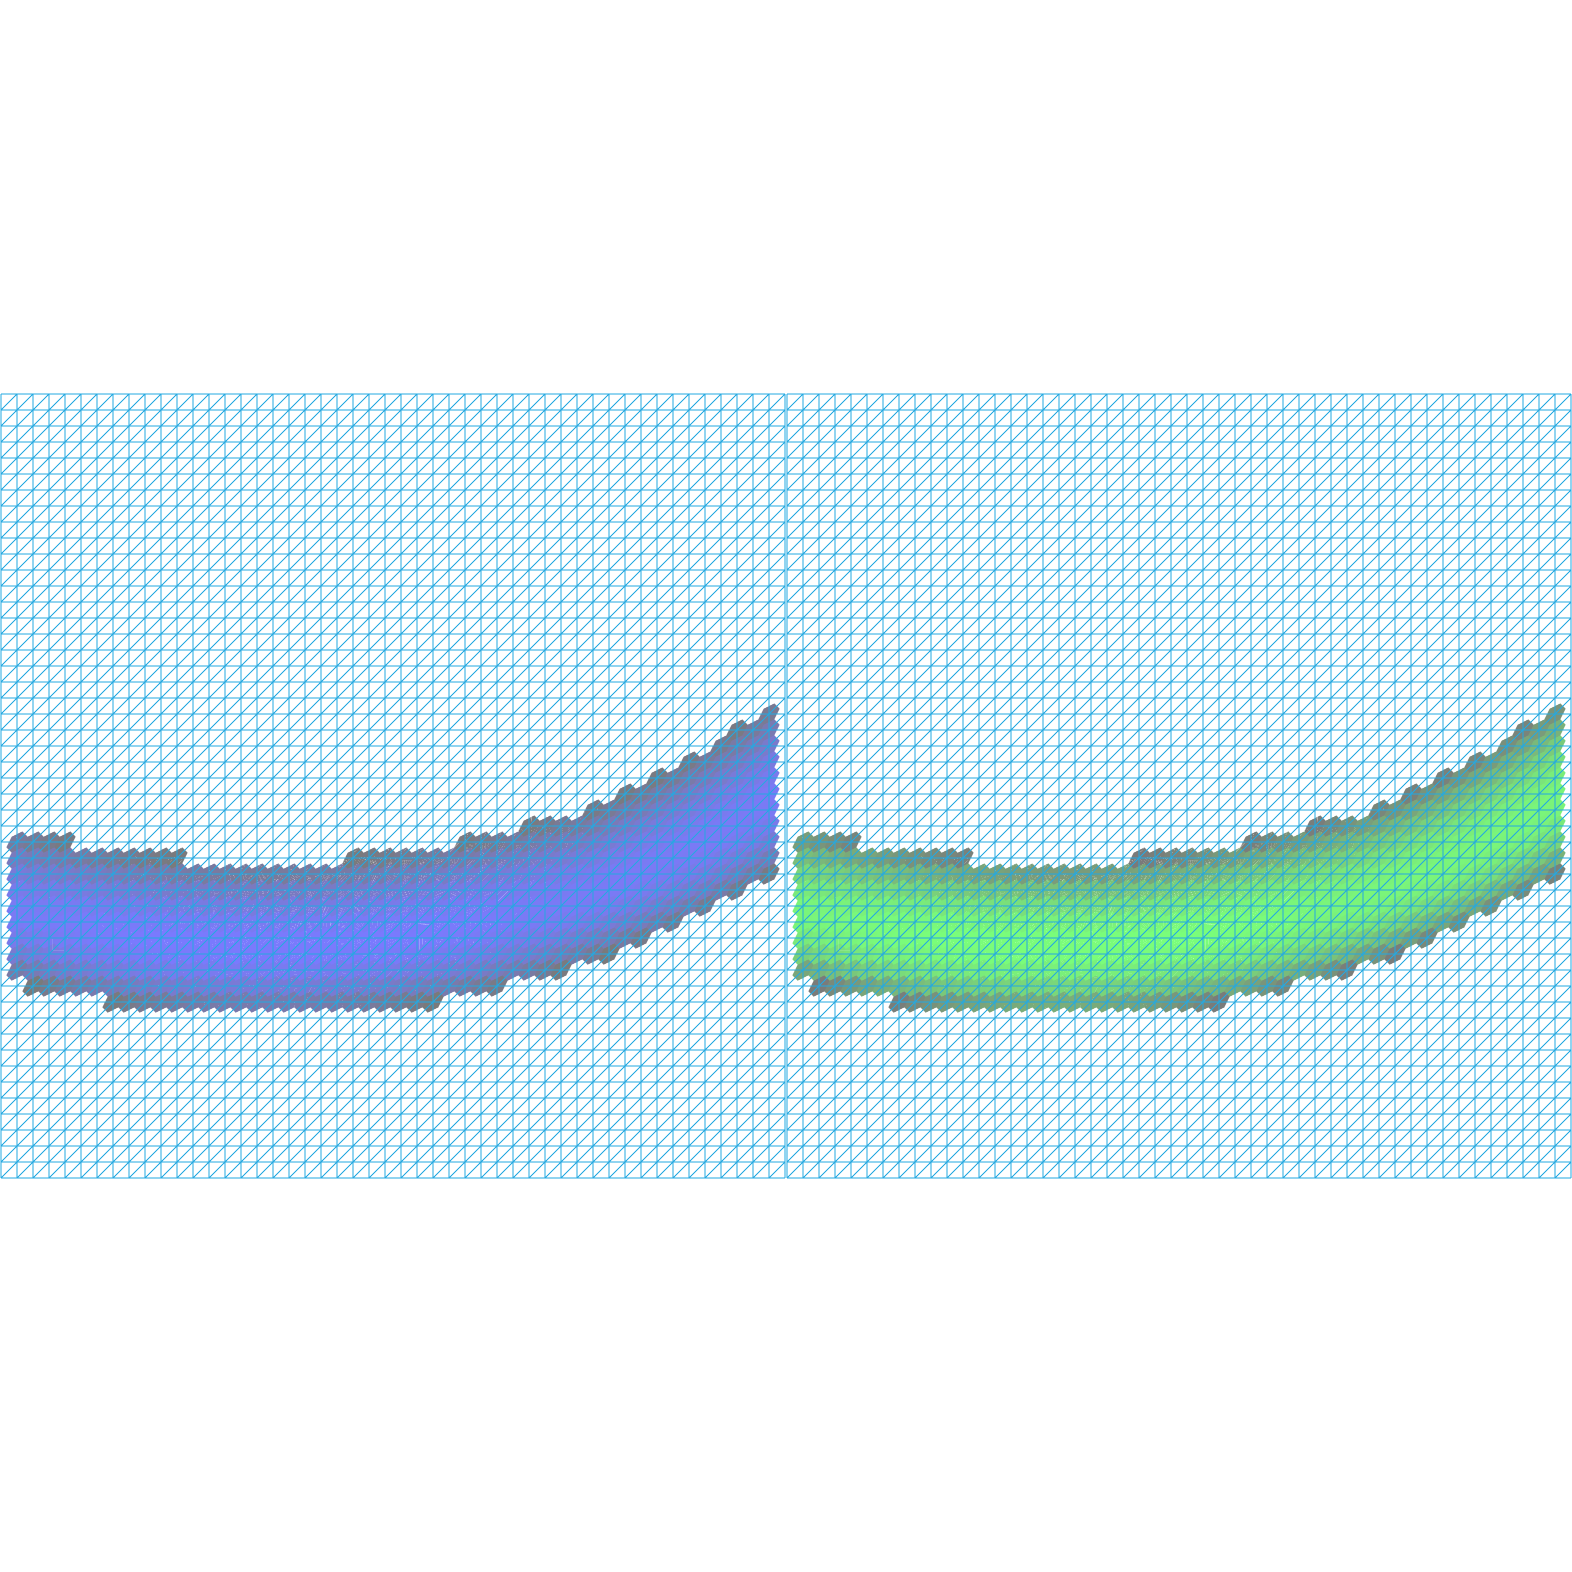
\includegraphics[width = 0.24\columnwidth]{figures/hill_exp/0_16/manipulability_comb_with_mesh_2}}
\subfigure[]{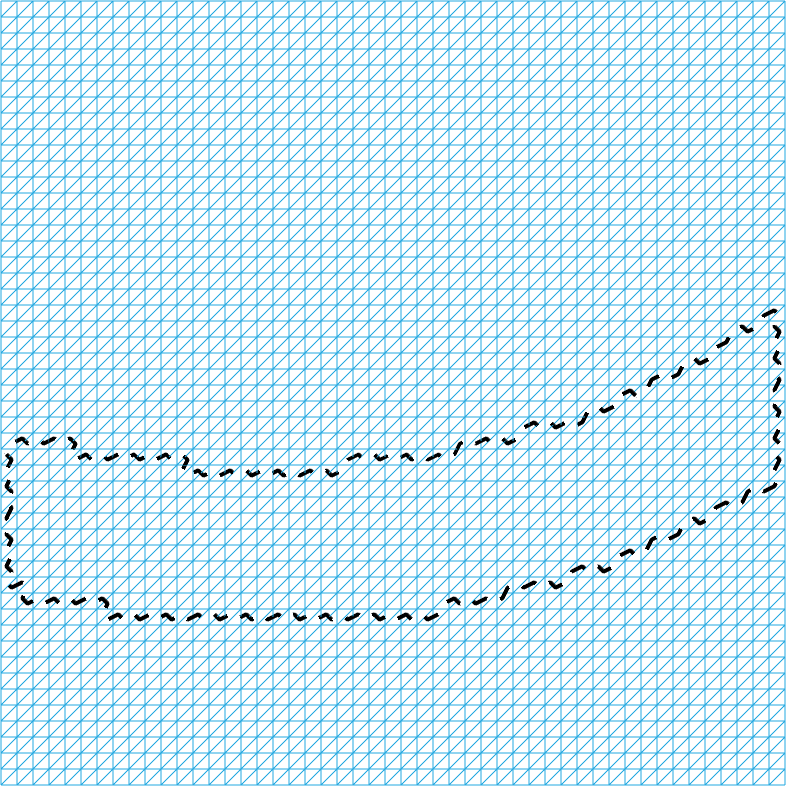
\includegraphics[width = 0.24\columnwidth]{figures/hill_exp/0_16/init_graph}}
\subfigure[]{\includegraphics[width = 0.24\columnwidth]{figures/hill_exp/0_16/result_graph}}
\caption{Like Fig.~\ref{fig_hill_exp_0_10}, where the threshold of manipulability is set to $> 0.16$. }
\label{fig_hill_exp_0_16}
\end{figure}


\section{Experimental Results}
\label{section_exp}
Several representative simulation works have been implemented to validate the proposed algorithm on challenging  arbitrarily-shaped objects.

% the optimal non-revisiting coverage planning path is solved. 
Fig. \ref{fig_mobius_exp} presents the solution of polishing a Mobi\"{u}s strip, whose surface is non-orientable. The manipulator is required to maintain the EE normal to the surface for proper operation simulating a contact task such as polishing. This is rather challenging in this case 
since the strip is twisted, hence the orientation of the normal vector varies over the full $2\pi$ rads. However, the proposed algorithm 
is able to come up with an configuration mapping leading to an optimal solution where only $1$ lift-off is required over the entire object.

Fig. \ref{fig_ring_exp} depicts the process of covering the surface of a ``swimming'' ring, another closed surface with no boundary. 
This is a particularly challenging case, it can be seen how the topological graph is formed by cells which are all multiply-connected, 
yet the proposed algorithm is able to come up with an effective solution with a single configuration discontinuity to the NCPP problem. 

The examples in Fig.~\ref{fig:hill_multiply_conn}, Fig.~\ref{fig_hill_exp_0_10} and Fig.~\ref{fig_hill_exp_0_16} illustrate the solutions of covering a ``hilly terrain" with varying degrees of desirable manipulability~\cite{yoshikawa1990translational}. 
For a given configuration (colour) cell, the manipulability is explicitly depicted brighter for increasing manipulability for the given configuration. The threshold  varies from a minium of $0.06$ (Fig.~\ref{fig:hill_multiply_conn}) to at least $0.10$ (Fig.~\ref{fig_hill_exp_0_10}), up to at least $0.16$, the maximum where a solution can be found for the object (in Fig.~\ref{fig_hill_exp_0_16}).

As one would expect, a sharp reduction on the reachable area is observed as the manipulability tightens 
(mainly due to the limited mobility of the wrist-flipped configurations, shown in the bottom two configurations 
in Fig.~\ref{fig:manip_010_configs}), causing large fluctuations in the structure of the resulting cells and topology graphs. When the threshold goes to $0.16$, most of the kinematic-valid wrist-unflipped configurations are no longer valid, as depicted in Fig.~\ref{fig_hill_exp_0_16}. % <jvm> Tong not sure if this should be the flipped or unflipped. Pls check here and also in the caption and text above just to make sure it is consistent with what we show in figures pls.
%However, in any case, our algorithm is applicable. 
%To sum up, for arbitrarily-shape objects, the optimal NCPP task on their surface can be transformed into the graph solving problem which is proved to be finitly solvable. 

\vfill

\section{Conclusion}
\label{section_conclusion}
This paper has proposed a theoretical complete solution to the optimal non-revisting coverage task problem of arbitrarily shaped objects with a non-redundant manipulator. 
Given topological graphs of surface cells corresponding to feasible and continuous manipulator configurations, 
the scheme ensures optimality with respect to the number of surface discontinuities, and is able to deal with non simply-connected 
space topologies, which arise for complex objects and as the number of task constraints limit the set of feasible configurations. 
%The proposed scheme effectively transforms the optimal CPP problem into an optimal colour designing problem of a topological configuration graph, which which has proven to be finitly solvable. 

In considering the generic solution to non simply-connected cells found in realistic 
environments, the proposed scheme effectively transforms the optimal CPP problem into an optimal colour designing problem of a topological configuration graph where a systematic solution for all genus cells is proposed. Through efficiently discarding equivalent and non-optimal cellular decompositions, the finiteness of divisions has been proven, and an upper bound in the number of divisions is calculated. 
%The detailed deduction of the complexity analysis and the extensive simulation are presented, suplemented by a video. 

Challenging simulation scenarios suplemented by a video are provided to validate the proposed scheme.
%A fast optimal cellular decomposition and a mechanism to generate optimal physical cellular decomposition are left for future works. 

\vfill

\section*{Acknowledgement}
This work was supported by National Key R\&D Program of China (2018YFB1309300) National Nature Science Foundation of China (61903332, U1609210).
The authors would like to thank Jin Gao for her careful examination on the formulae proposed in this paper. 

\vfill

\begin{comment}
However, due to the lack of considerations of weird constraints appearing in realistic environment, the proved finiteness of different cellular decompositions and the proposed solutions are valid only for the simply-connected cells. 
And there is no criterion about the environment settings and the constraints that describes the applicability of the proposed algorithm. 
Besides the kinematic, the static force and the manipulability constraints considered in~\cite{Yang2020Cellular}, given more complicated constraints and strange thresholds, the emergence of the non simply-connected cells is inevitable. 

Since the structure of all cells appearing in the graph can be classified through the genus, i.e., number of ``holes" within their outer contour, the problem is completely solved as long as the cells with arbitrary genus are proved finitely solvable and nominated a solution. 
\end{comment}



%% Use plainnat to work nicely with natbib. 

\newpage % <jvm> this should be on page 9

\bibliographystyle{plainnat}
\bibliography{min_removal_RSS}

\end{document}


